%$Id $
\documentclass[11pt,a4paper,twoside,openright]{report}
\usepackage[utf8]{inputenc}
\usepackage[spanish]{babel}
\usepackage{graphicx}
\usepackage{multicol}
\usepackage{balance}

\usepackage{textcomp}
\usepackage{amsmath}
\usepackage{mathtools}
\usepackage{caption}
\usepackage{subcaption}
\usepackage{multirow}
\usepackage{multicol}
\usepackage{array}
\usepackage{listings}

\lstset{
  basicstyle=\ttfamily\footnotesize,%\scriptsize,
  language=C,
  keywordstyle=\bfseries,
  breaklines=true,
  keywords=[2]{INT8U,INT16U,DIO\_DI,DIO\_DO,CPU\_INT16S,CPU\_INT08U}
}

\lstset{literate=
  {á}{{\'a}}1 {é}{{\'e}}1 {í}{{\'i}}1 {ó}{{\'o}}1 {ú}{{\'u}}1
  {Á}{{\'A}}1 {É}{{\'E}}1 {Í}{{\'I}}1 {Ó}{{\'O}}1 {Ú}{{\'U}}1
  {à}{{\`a}}1 {è}{{\'e}}1 {ì}{{\`i}}1 {ò}{{\`o}}1 {ù}{{\`u}}1
  {À}{{\`A}}1 {È}{{\'E}}1 {Ì}{{\`I}}1 {Ò}{{\`O}}1 {Ù}{{\`U}}1
  {ä}{{\"a}}1 {ë}{{\"e}}1 {ï}{{\"i}}1 {ö}{{\"o}}1 {ü}{{\"u}}1
  {Ä}{{\"A}}1 {Ë}{{\"E}}1 {Ï}{{\"I}}1 {Ö}{{\"O}}1 {Ü}{{\"U}}1
  {â}{{\^a}}1 {ê}{{\^e}}1 {î}{{\^i}}1 {ô}{{\^o}}1 {û}{{\^u}}1
  {Â}{{\^A}}1 {Ê}{{\^E}}1 {Î}{{\^I}}1 {Ô}{{\^O}}1 {Û}{{\^U}}1
  {œ}{{\oe}}1 {Œ}{{\OE}}1 {æ}{{\ae}}1 {Æ}{{\AE}}1 {ß}{{\ss}}1
  {ç}{{\c c}}1 {Ç}{{\c C}}1 {ø}{{\o}}1 {å}{{\r a}}1 {Å}{{\r A}}1
  {€}{{\EUR}}1 {£}{{\pounds}}1 {"}{{``}}1
}

\renewcommand{\lstlistingname}{Código}
\addto\captionsspanish{\renewcommand{\chaptername}{Sección}}
\newcommand{\HRule}{\rule{\linewidth}{0.5mm}}

\usepackage{color}
\usepackage{pxfonts}
\usepackage{dirtree}
\usepackage{verbatim}

%\usepackage{subfig}
%\usepackage[cm]{fullpage}
\usepackage[a4paper]{geometry}
%\usepackage{subfigure}
\usepackage{float}
\usepackage{fancyhdr}
\usepackage{caption}
\usepackage{subcaption}

% \title{Proyecto Final de \emph{Software en Tiempo Real} \\ \small{Sistema con sensor controlador por una línea serial}}
% \author{Luis A. Guanuco}
%\date{Febrero 2014}


\pagestyle{fancy}
\addtolength{\textheight}{2cm}
%\addtolength{\voffset}{-1cm}
%\addtolength{\textwidth}{1cm}

% -------------- Define --------------
\def\uCOS{$\mu$C/OS-II\texttrademark}

% -------------- Re-definición de comandos/macros --------------
\renewcommand\spanishtablename{Tabla}   %Table (for caption)

\begin{document}

\begin{titlepage}
\begin{center}

\textsc{\LARGE Universidad Tecnológica Nacional}\\[0.5cm]
\textsc{\LARGE Facultad Regional Córdoba}\\[2cm]


\includegraphics[width=0.1\textwidth]{images/logoUTN}~\\[2cm]

\textsc{\Large Proyecto Final de \emph{Software en Tiempo Real}}\\[0.5cm]

% Title
\HRule \\[0.4cm]
{ \huge \bfseries Sistema con sensor controlador por una línea serial \\[0.4cm] }

\HRule \\[1.5cm]

% Author and supervisor
\begin{minipage}{0.4\textwidth}
\begin{flushleft} \large
\emph{Alumno:}\\
Luis Alberto \textsc{Guanuco}
\end{flushleft}
\end{minipage}
\begin{minipage}{0.4\textwidth}
\begin{flushright} \large
\emph{Docentes:} \\
Ing.~Carlos \textsc{Centeno} \\
Ing.~Luis \textsc{Toledo} 
\end{flushright}
\end{minipage}

\vfill

% Bottom of the page
{\large \today}

\end{center}
\end{titlepage}

%\maketitle{}

\tableofcontents{}
\listoffigures{}
\listoftables{}

\lhead{Luis A. Guanuco}
%\chead{
\includegraphics[width=0.02\textwidth]{images/logoUTN}}
\rhead{Proyecto Final de \emph{Software en Tiempo Real}}


% \begin{figure}[h]
%   \centering
%   
\includegraphics[width=0.1\textwidth]{images/logoUTN}
% \end{figure}


\begin{abstract}
  El presente trabajo se enfocada en la implementación de un sistema de comunicación sobre una red serial donde se encuentran conectados un sensor, un sistema electrónico con un microcontrolador y por último se conecta una computadora personal (PC). Los sistemas electrónicos basados en un procesador poseen un Sistema Operativo en Tiempo Real, RTOS por sus siglas en inglés (\textsl{Real-Time Operating Systems}). El sensor presenta una particularidad, y es que tanto la alimentación del transductor como el canal de datos es el mismo. Los parámetros principales en el diseño son definidos por el circuito del sensor.
\end{abstract}

\chapter{Introducción}
\label{sec:intro}

La posibilidad de reducir el costo en cualquier sistema electrónico es uno de los grandes retos con el que se presenta el desarrollador electrónico. Si bien hay un gran avance en los procesos de fabricación de circuitos integrados, existen dos inconvenientes para hacerse de dicha tecnología. El primero es el \emph{acceso} a los nuevos dispositivos electrónicos que se encuentran en el mercado. El segundo inconveniente que se podría enumerar, muy relacionado al primero, es el \emph{costo} que tienen estos nuevos dispositivos. Obviamente que estos inconvenientes planteados son desde un perfil estudiantil. Seguramente en desarrollos industriales los factores de disponibilidad y costo son evaluados en función de las prestaciones que ofrece el dispositivo en cuestión. Pero como nuestro trabajo se encuentra orientado a un ámbito académico se priorizará el diseño que requiera mayor tiempo de investigación y desarrollo para obtener un sistema que cumpla con nuestros requerimientos a un costo reducido y que pueda ser reproducible fácilmente.

El procesamiento de datos se realizará sobre un dispositivo microcontrolador dsPIC\textsuperscript{\textregistered}  fabricado por Microchip Inc.. En este $\mu$C se encuentra embebido un RTOS donde se implementan varias tareas para el sistema operativo (OS). Debido a la complejidad del desarrollo, a nivel de \textsl{software}, no se presentan problemas en los tiempos de procesamiento del OS. Como se dijo en el Resumen del informe, las principales especificaciones son propias del sistema transductor (sensor).

La información relevada por el sistema embebido es transmitida a una PC, quién presentará la información obtenida del sensor. Siguiendo la línea del uso sistemas operativos en tiempo real, se implementa nuevamente un RTOS. Al igual que en el caso del dsPIC\textsuperscript{\textregistered}, aquí se adaptan la capa más baja del código máquina para compilar el sistema operativo con la arquitectura a utilizar. La mayoría de la información necesaria para esta \emph{adaptación} se encuentra disponible por el desarrollador del RTOS (Micri$\mu$m Inc.).

\chapter{Especificaciones del diseño}
\label{sec:esp-diseno}

Las especificaciones del desarrollo se las puede dividir en dos grupos. Por un lado especificaciones de \emph{Hardware}, aquí se encuentra tanto el circuito del sensor como así también la plataforma de procesamiento y los recursos disponibles. Por otro lado se especifica el \emph{Software} que se debe implementar, el sistema operativo en tiempo real \uCOS. Ya familiarizado por el desarrollador del proyecto por ser el OS utilizado en la \emph{Cátedra de Software en Tiempo Real} dictado como materia electiva en la Carrera Ingeniería Electrónica de la Universidad Tecnológica Nacional -- Facultad Regional Córdoba.

\section{\textsl{Hardware}}
\label{sec:esp-hw}

El esquema general del \textsl{hardware} se puede ver en la Fig. \ref{fig:hw-esquema}. Aquí se especifica el flujo de dato entre los diferentes bloques. Sobre las líneas de comunicación se tiene comentado que información dispone físicamente cada conexión. En la conexión entre el sensor y el dsPIC\textsuperscript{\textregistered} se no solo se comparte información (datos) sino también se transmite energía para el circuito transductor. Entre el dsPIC\textsuperscript{\textregistered} y la PC se implementa una comunicación RS-232.

\begin{figure}[h]
  \centering
  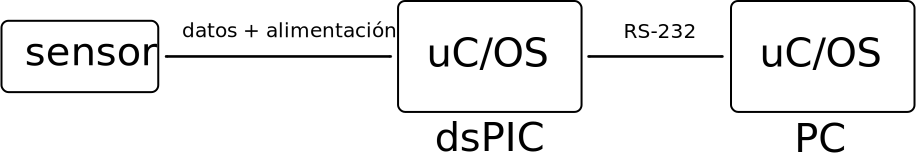
\includegraphics[width=0.6\textwidth]{images/hw-esquema-gral}  
  \caption{Esquema general de la implementación.}
  \label{fig:hw-esquema}
\end{figure}

\section{\textsl{Software}}
\label{sec:esp-sw}

Como se mencionó anteriormente, tanto en el dsPIC\textsuperscript{\textregistered} como en el PC se implementan el sistema operativo \uCOS. Si bien las especificaciones a nivel \textsl{hardware} no demanden el uso de un RTOS, ya que los requerimientos en la respuesta del procesamiento no son críticas, se hará uso de estos sistemas operativos como una aplicación de las características mas destacadas con la que cuentan los RTOS (\uCOS en nuestro caso). 
En las secciones siguientes se describirá con mayor detalle tanto el \textsl{hardware} como el \textsl{software}. 

\chapter{Implementación del circuito electrónico}
\label{sec:circ}

A nivel electrónico, el desarrollo se divide en dos diseños. El primero es el circuito de sensor y el segundo es el sistema embebido con el dsPIC\textsuperscript{\textregistered} como dispositivo principal.

\section{Circuito del sensor}
\label{sec:circ-sensor}

La base del circuito transductor es un oscilador forma por un inversor digital (IC) y una red RC que determina la frecuencia de oscilación del oscilador. Para mantener más estable la frecuencia del oscilador se utiliza un inversor \emph{Schmitt-Trigger}. Esto último se debe a que el sistema sensor presentará algunas perturbaciones en el nivel de la tensión de alimentación, causa que se abordará más adelante en esta sección. La transducción del fenómeno físico que se quiere adquirir se producirá afectado la red RC, es decir la frecuencia del oscilador. Por la disponibilidad de transductores discretos, se opta por usar un sensor fotoeléctrico ó LDR (por sus siglas en inglés \textsl{Light Dependant Resistor}). 

\subsection{Oscilador \textsl{Schmitt-Trigger}}
\label{sec:osc-schmitt}

El oscilador basado con un inversor es un circuito muy sencillo que demanda el uso de una red formada por un resistor y un capacitor, ilustrado en la Figura \ref{fig:schmitt-circuito}. El inversor utilizado en este caso es el \textbf{MM74HCT14}\footnote{Se puede utilizar cualquier otro integrado con inversores pero debe contar con la tecnología \textsl{Schmitt-Trigger}.}, el cual dispone de ocho inversores con \textsl{Schmitt-Trigger}. El concepto sobre de \textsl{Schmitt-Trigger} fue inventado por el científico estadounidense \emph{Otto H. Schmitt} en el año 1934. Se lo llama \emph{Trigger} pues la salida del circuito retiene su estado hasta que la entrada presenta un valor suficiente para disparar (en inglés \textsl{trigger}) en cambio de estado. En la Figura \ref{fig:schmitt-tiempo} se observa los niveles umbrales de tensión (\textsl{threshold}) que presenta este tipo de inversor. El comportamiento dinámico de ambos niveles umbrales se lo puede graficar como un ciclo de histéresis (Figura \ref{fig:schmitt-histeresis}), este comportamiento permite decir el \textsl{Schmitt-Trigger} posee \emph{memoria} y puede actuar como un circuito biestable (latch o flip-flop). Aunque su principal uso es el acondicionamiento de señales digitales, permitiendo remover el ruido en la señal.

\begin{figure}[H]
  \begin{subfigure}[b]{0.2\textwidth}
    \centering
    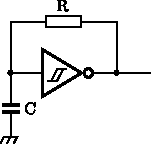
\includegraphics[width=\textwidth]{images/schmitt_trigger_circuito}
    \subcaption{Oscilador}\label{fig:schmitt-circuito}
  \end{subfigure}
  \hfill
  \begin{subfigure}[b]{0.35\textwidth}
    \centering
    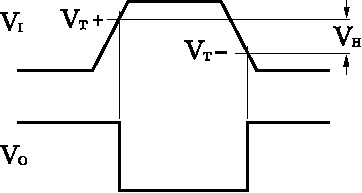
\includegraphics[width=\textwidth]{images/schmitt_trigger_tiempo}
    \subcaption{Diagrama de tiempo}\label{fig:schmitt-tiempo}
  \end{subfigure}  
  \hfill
  \begin{subfigure}[b]{0.25\textwidth}
    \centering
    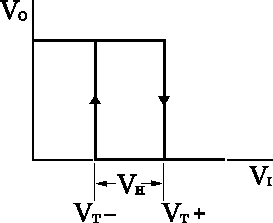
\includegraphics[width=\textwidth]{images/schmitt_trigger_histeresis}    
    \subcaption{Histéresis}\label{fig:schmitt-histeresis}
  \end{subfigure}  
  \caption{Circuito con \textsl{Schmitt-Trigger}.}
\end{figure}

La frecuencia de oscilación del circuito implementado en la Figura \ref{fig:schmitt-circuito} es determinado por el valor de los componentes pasivos ($RC$), el nivel de la tensión de alimentación $V_{CC}$, y los niveles umbrales $V_{T+}$ y $V_{T-}$. La ecuación (\ref{eq:freq-osc}) se obtuvo desde una nota de aplicación del integrado a utilizar. 

\begin{equation}
  \label{eq:freq-osc}
  \begin{array}[h]{r c l}
    f & \approx & 1\over {RC\ln\left[{V_{T+}\left(V_{CC}-V_{T-}\right)}\over{V_{T-}\left(V_{CC}-V_{T+}\right)}\right]}\\
    f & \approx & 1\over {RCk}\\
  \end{array}
\end{equation}

La ecuación (\ref{eq:freq-osc}) demuestra que puede considerarse como una constante $k$ la operación logarítmica para facilitar la estimación de la frecuencia a la que oscila el circuito con el inversor. Se podría representar el comportamiento del valor constante $k$ como una curva donde se considerará variaciones en el valor de la tensión de alimentación $V_{CC}$. La Figura \ref{fig:ctte-k} demuestra que es posible mantener estable la frecuencia aun con variaciones significativas en la tensión de alimentación. Más adelante se especificará como influye esto en nuestro caso, sobre todo por la particularidad de que nuestro sistema será sometido a perturbaciones intencionales en el nivel de alimentación.

\begin{figure}[h]
  \centering
  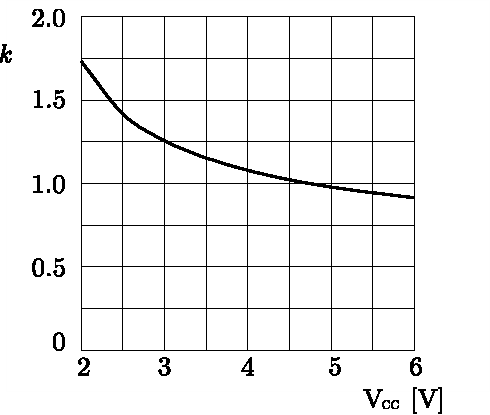
\includegraphics[width=0.6\textwidth]{images/constante-k}
  \caption{Curva $V_{CC}$ vs. $k$.}
  \label{fig:ctte-k}
\end{figure}

\subsection{Funcionamiento básico}
\label{sec:funcionamiento}

En la sección anterior se describe el funcionamiento del oscilador basado en un circuito con un inversor. En este circuito la frecuencia de oscilación, ecuación (\ref{eq:freq-osc}), es inversamente proporcional al producto $RCk$. Aquí vamos a considerar que tanto $C$ como $k$ son constantes, el parámetro que determinará la frecuencia es el valor de $R$. El resistor $R$ es en nuestro caso el transductor LDR. Este transductor varía su parámetro de resistividad en función de la cantidad de luz que incida sobre él. Un esquema del proceso de conversión de variables se puede ver en la Figura \ref{fig:proceso-sensor}.

\begin{figure}[h]
  \centering
  \includegraphics[width=0.6\textwidth]{images/proceso_sensor}
  \caption{Proceso de conversión de variables en el sistema de censado.}
  \label{fig:proceso-sensor}
\end{figure}

En función a lo anteriormente dicho, se debe adquirir y procesar una onda oscilante donde la información se encuentra en el frecuencia que dicha señal posee. Además se especifica que \emph{no se considerarán variaciones bruscas} en la intensidad de la luz recibida por el LDR. Para determinar los rangos máximos y mínimos en la variación de la resistividad del LDR se realizaron algunas mediciones que se pueden ver en la Tabla \ref{tab:rango-ldr}.

\begin{table}[h]
  \centering
  \begin{tabular}[h]{|c|c|}
    \hline
    \textbf{Condición de Luz} & \textbf{Valor de resistividad} \\
    \hline
    Oscuridad & 180 K$\Omega$ \\
    \hline
    Claridad & 1 K$\Omega$ \\
    \hline
  \end{tabular}
  \caption{Rango de variación del LDR.}
  \label{tab:rango-ldr}
\end{table}

Con la información del rengo resistivo del LDR se puede definir el rango de frecuencias de la señal que se obtendrá del sensor oscilador. Otra especificación a tener en cuenta es la frecuencia de muestreo que dispone el bloque siguiente al sensor, el microcontrolador dsPIC\textsuperscript{\textregistered}. Aquí se tiene que el tiempo de muestreo es de 100 $\mu$S.. Según el teorema del muestreo de Nyquist-Shannon, se podría definir un límite en la frecuencia máxima posible a ser adquirida. El enunciado de este teorema dice,

\begin{equation}
  \label{eq:nyquist}
  \begin{array}[h]{c c c c}
      F_{S} & > & 2F_{M\acute{A}X} & \text{, donde } F_{M\acute{A}X} \text{ es la frecuencia máxima de la señal.} \\
  \end{array}
\end{equation}

en función a esta definición, se puede encontrar cual será la frecuencia máxima que se detectará correctamente si la frecuencia de muestreo es de 100 $\mu$S. Es decir,

\begin{equation}
  \label{eq:freq-max}
  \begin{array}[h]{l c c c c l}
    \text{sí}       &    F_{S}        & > &    2F_{M\acute{A}X}         &     &         \\\vspace{0.2cm}
    \text{entonces} &    F_{M\acute{A}X} & < &    {F_{S}} \over 2       &     &         \\\vspace{0.2cm}
                    &    F_{M\acute{A}X} & < &    1 \over {2T_{S}}      &     &         \\\vspace{0.2cm}
                    &    F_{M\acute{A}X} & < &    1 \over {2\,100\mu S}&  =  &  5 KHz  \\
  \end{array}
\end{equation}

Una vez obtenida la máxima frecuencia que se puede reconocer por parte del sensor, conjuntamente con los valores de resistividad (Tabla \ref{tab:rango-ldr}), se realizan ensayos para determinar el valor que debe tener el capacitor de la red $RC$ del oscilador\footnote{Se considera $k = 1$}. En la Tabla \ref{tab:freq-dif-cap} se muestran dos configuraciones diferentes para distintos valores de capacitancia (10 nF y 100 nF).

\begin{table}[h]
  \centering
  \begin{tabular}[h]{|r|r|r|}
    \hline
    \textbf{Capacitor} & \textbf{Rango del LDR [$\Omega$]} & \textbf{Frecuencia del osc.} \\
    \hline
    \multirow{2}{*}{10 nF}  & 1 K$\Omega$   & 100 KHz \\
                            & 180 K$\Omega$ & 555 Hz  \\
    \hline
    \multirow{2}{*}{100 nF} & 1 K$\Omega$   & 10 KHz  \\
                            & 180 K$\Omega$ & 55 Hz   \\
    \hline
  \end{tabular}
  \caption{Rango de frecuencias de salida en función de la red $RC$.}
  \label{tab:freq-dif-cap}
\end{table}

En función a la Tabla \ref{tab:freq-dif-cap} se puede decir que el valor de capacidad más apropiado es \emph{100 nF}. Pues con este valor se tiene un rango de frecuencia aceptable para la frecuencia de muestreo de 100 $\mu$s. 

Una \emph{características importante} del circuito planteado en este trabajo es la posibilidad de \emph{reutilizar} la línea de comunicación como canal de alimentación. El circuito a utilizar se presenta en la Fig. \ref{fig:hw-placa-sensor}. En el esquema de conexión se destacan dos componentes que son responsables de mantener el nivel de tensión de alimentación, el capacitor electrolítico $C1$ y el diodo $D1$. El capacitor electrolítico almacenará carga recibida de la línea serial, direccionada por $D1$. En el momento que la línea baje su nivel de tensión, el capacitor proporcionará la corriente al circuito inversor, obviamente que lo hará por un tiempo reducido ya que comenzará a descargarse. El resistor $R2$ permite aumentar la impedancia de la salida del invesor (TTL). 

\begin{figure}[ht]
  \centering
  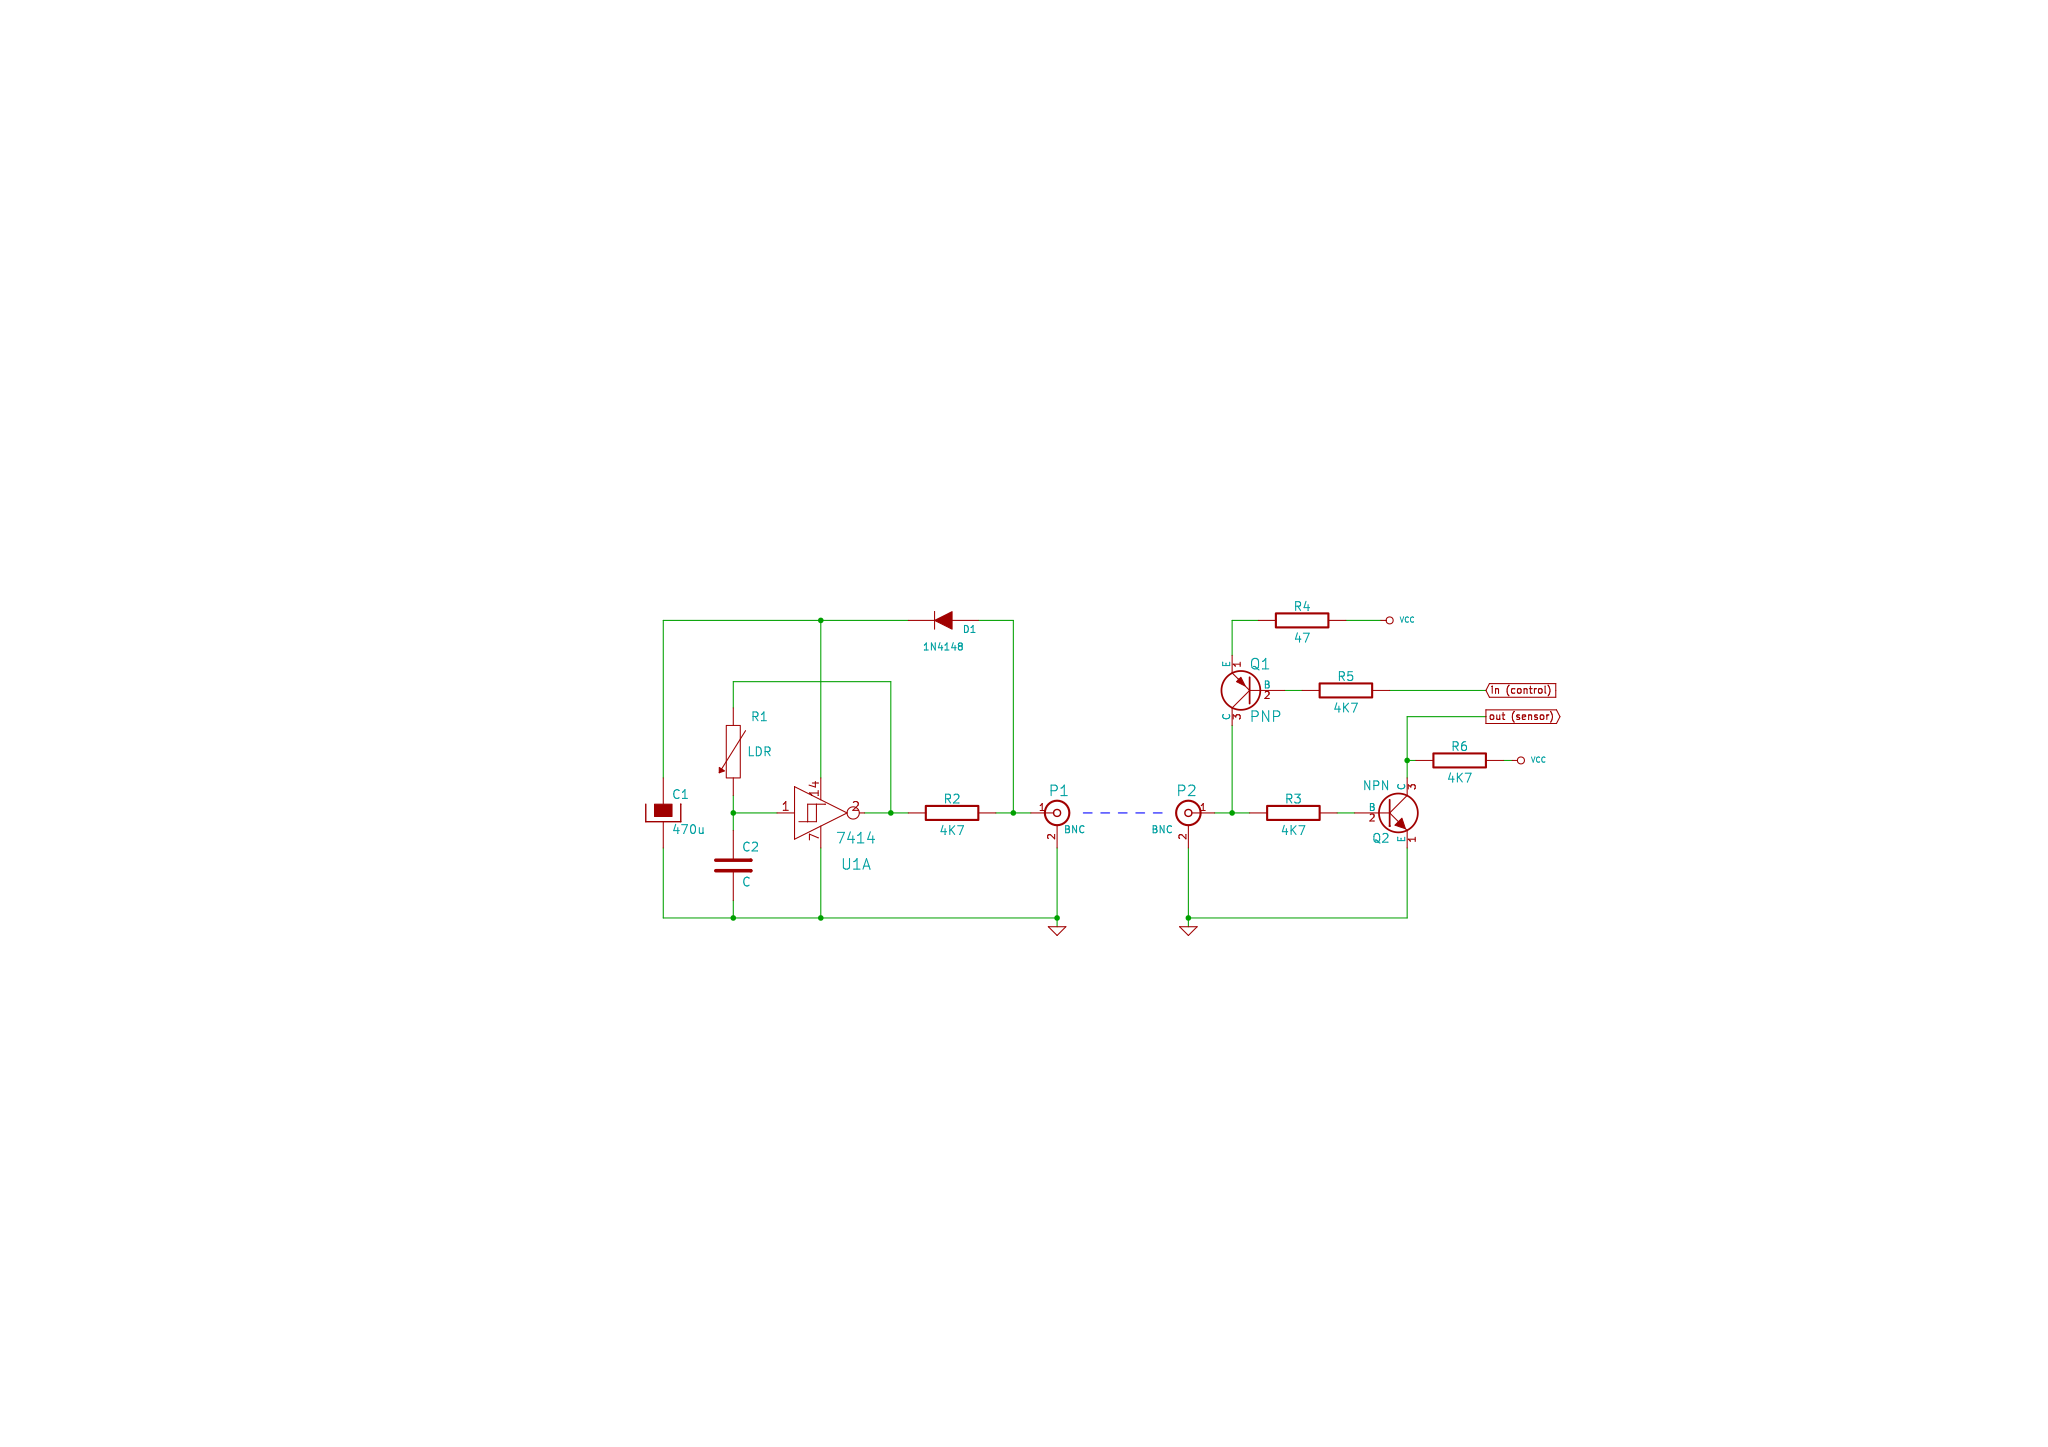
\includegraphics[width=0.8\textwidth]{images/placa_sensor}
  \caption{Implementación del circuito electrónico.}
  \label{fig:hw-placa-sensor}
\end{figure}

La línea de comunicación/alimentación conecta el circuito del sensor (del lado izquierdo de la Figura \ref{fig:hw-placa-sensor}) con el circuito de control del sistema (a la derecha del la figura). El sistema de control es muy sencillo y cuenta de solo dos secuencias. 
\begin{description}

\item[Mode de espera,]  este modo consiste en mantener la línea a un nivel de tensión necesario para alimentar el circuito del sensor (inversor). Para esta situación se debe enviar una señal de control a la base del transistor $Q1$. La señal $in (control)$ proviene del dsPIC\textsuperscript{\textregistered}, controlador por el RTOS, que veremos en las siguientes secciones. Si la señal presenta un $0$ lógico el transistor PNP se polarizará y la línea quedará conectada a la tensión $V_{CC}$. La señal de salida $out (sensor)$ tendrá el mismo nivel que la línea ($V_{CC}$) ya que el transistor $Q2$ está polarizado con la señal de la línea. 

\item[Modo adquisición,] la adquisición de la señal oscilante que genera el circuito inversor es transmitida cuando la línea es liberada por el transistor $Q1$. En el momento que se presenta un $1$ en la señal de control de $Q1$, éste queda abierto. Por una lado, el \textsl{Schmitt-trigger} deja de ser alimentado por la línea pero recibe carga del capacitor $C1$. Por otro lado la señal generada por le oscilador es transmitida a la línea que será amplificada por el transistor $Q2$. Si bien la señal del oscilador podría encontrarse debilita por pérdidas en la línea, el circuito de $Q2$ permite polarizar con niveles bajos de corriente el transistor NPN.

\end{description}

Esta secuencia debe mantener una relación entre el \emph{ciclo de adquisición} y \emph{ciclo de espera}. Por ejemplo, un ciclo de adquisición muy largo provocará una elevada reducción en la tensión de alimentación del inversor que, en este ciclo, es proporcionado por el capacitor $C1$. En caso contrario, un ciclo de adquisición muy corto podría no registrar el ciclo completo de oscilación del sensor. Una relación que se consideró apropiada es $^1/_{10}$, para un ciclo completo de control $T$ el tiempo de adquisición se toma $^1/_T$ y el tiempo de espera $^9/_T$. La representación temporal de este proceso se puede ver en la Figura \ref{fig:ciclo-tiempo}.

\begin{figure}[H]
  \begin{subfigure}[b]{\textwidth}
    \centering
    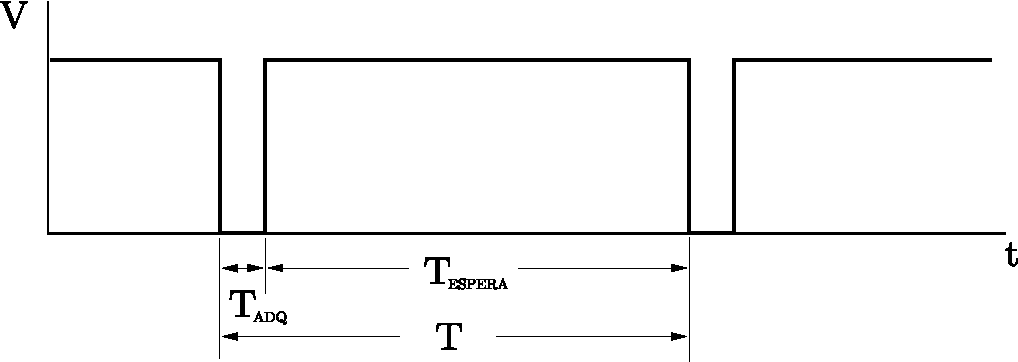
\includegraphics[width=0.65\textwidth]{images/ciclo_tiempo_control}
    \subcaption{Señal de control (Base del transistor $Q1$)}\label{fig:ciclo-control}
  \end{subfigure}
  \hfill
  \begin{subfigure}[b]{\textwidth}
    \centering
    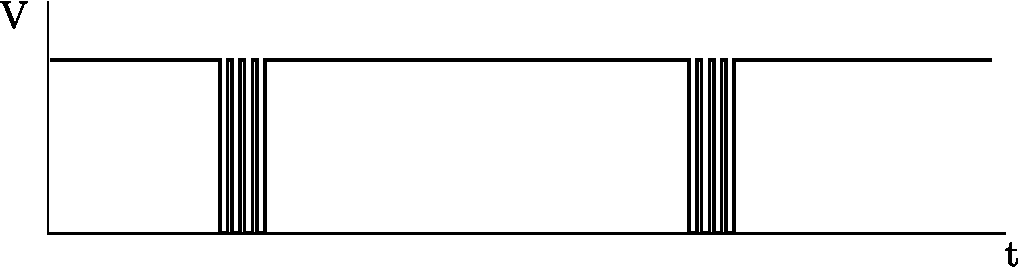
\includegraphics[width=0.65\textwidth]{images/ciclo_tiempo_linea}
    \subcaption{Señal en la línea (Colector $Q1$ / Base $Q2$)}\label{fig:ciclo-linea}
  \end{subfigure}  
  \hfill
  \begin{subfigure}[b]{\textwidth}
    \centering
    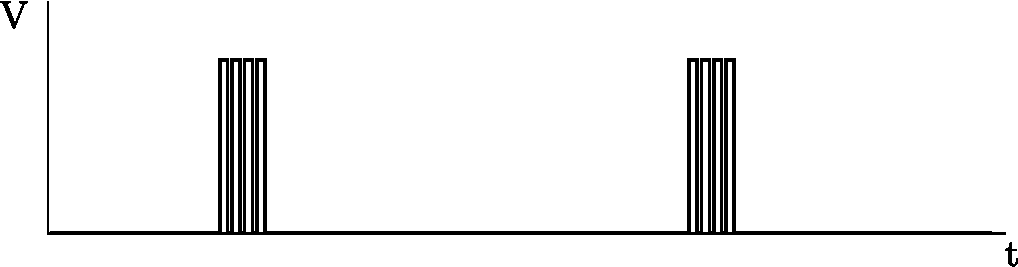
\includegraphics[width=0.65\textwidth]{images/ciclo_tiempo_salida}    
    \subcaption{Señal de salida (Colector del transistor $Q2$)}\label{fig:ciclo-salida}
  \end{subfigure}  
  \begin{subfigure}[b]{\textwidth}
    \centering
    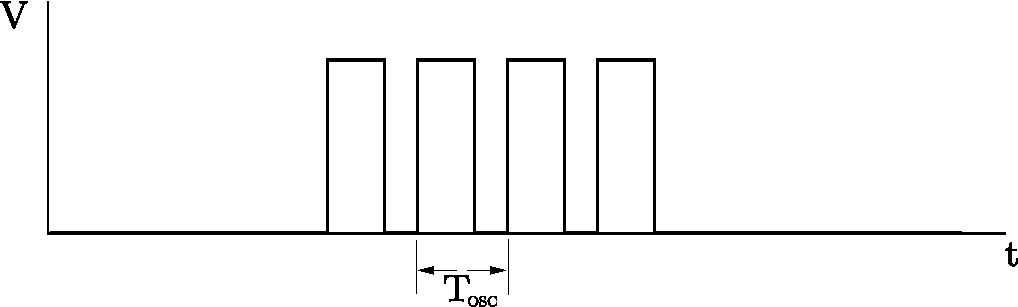
\includegraphics[width=0.65\textwidth]{images/ciclo_tiempo_salida_zoom}    
    \subcaption{Señal de salida amplificada de la figura (\subref{fig:ciclo-salida})}\label{fig:ciclo-salida-zoom}
  \end{subfigure}  
  \caption{Diagramas temporales de los ciclos de Espera y Adquisición.}
  \label{fig:ciclo-tiempo}
\end{figure}

\section{Circuito del dsPIC\textsuperscript{\textregistered}}
\label{sec:circ-dspic}

Para realizar el proceso de control del sistema de censado se utiliza un microcontrolador del fabricante Microchip, el DSPIC33FJ128GP804-E/PT. Este dispositivo presenta enormes prestaciones en recursos de \textsl{hardware}, aquí se presentan algunos de ellos:

\begin{itemize}

\item [] \textbf{Clock Management}
  \begin{itemize}
  \item  2\% internal oscillator                        
  \item  Programmable PLL and oscillator clock sources 
  \item  Fail-Safe Clock Monitor (FSCM)                
  \item  Independent Watchdog Timer                    
  \item  Low-power management modes                    
  \item  Fast wake-up and start-up                     
  \end{itemize}

\item [] \textbf{Core Performace}
  \begin{itemize}
  \item  Up to 40 MIPS 16-bit dsPIC33F CPU    
  \item  Single-cycle MUL plus hardware divide
  \end{itemize}

\item [] \textbf{Communication Interfaces}
  \begin{itemize}
  \item  Parallel Master Port (PMP)                                  
  \item  Two UART modules (10 Mbps)
    \begin{itemize}
    \item [-] Supports LIN 2.0 protocols                              
    \item [-] RS-232, RS-485, and IrDA\textsuperscript{\textregistered} support                       
    \end{itemize}
  \item  Two 4-wire SPI modules (15 Mbps)                            
  \item  Enhanced CAN (ECAN) module (1 Mbaud) with 2.0B support      
  \item  I2C module (100K, 400K and 1Mbaud) with SMbus support       
  \item  Data Converter Interface (DCI) module with I2S codec support
\end{itemize}

\item [] \textbf{System Peripherals}
  \begin{itemize}
  \item  16-bit dual channel 100 ksps Audio DAC                 
  \item  Cyclic Redundancy Check (CRC) module                   
  \item  Up to five 16-bit and up to two 32-bit Timers/Counters 
  \item  Up to four Input Capture (IC) modules                  
  \item  Up to four Output Compare (OC) modules                 
  \item  Real-Time Clock and Calendar (RTCC) module             
\end{itemize}

\item [] \textbf{Advanced Analog Features}
\begin{itemize}
\item 10/12-bit ADC with 1.1Msps/500 ksps rate:
  \begin{itemize}
  \item [-] Up to 13 ADC input channels and four S\&H
  \item [-] Flexible/Independent trigger sources
  \end{itemize}
\item 150 ns Comparators:
  \begin{itemize}
  \item [-] Up to two Analog Comparator modules
  \item [-] 4-bit DAC with two ranges for Analog Comparators
  \end{itemize}
\end{itemize}

\item [] \textbf{Input/Output}
  \begin{itemize}
  \item Software remappable pin functions          
  \item 5V-tolerant pins                           
  \item Selectable open drain and internal pull-ups
  \item Up to 5 mA overvoltage clamp current/pin   
  \item Multiple external interrupts                   
  \end{itemize}

\item [] \textbf{Direct Memory Access (DMA)}
  \begin{itemize}
  \item 8-channel DMA with no CPU stalls or overhead
  \item UART, SPI, ADC, ECAN, IC, OC, INT0
  \end{itemize}

\item [] \textbf{Debugger Development Support}
  \begin{itemize}
  \item In-circuit and in-application programming
  \item Two program breakpoints
  \item Trace and run-time watch
  \end{itemize}
  
\end{itemize}
            
La placa de desarrollo de este microcontrolador es un diseño realizado por estudiantes de nuestra casa de estudios \emph{Andrés Hoc} y \emph{Gonzalo Vassia}\footnote{Los estudiantes realizaron la placa con la finalidad de disponer un diseño sencillo y flexible para múltiples propósitos.}, Figura \ref{fig:circuito-dspic}. Para la programación de este microcontrolador se utilizó el entorno de desarrollo \emph{MPLAB\textsuperscript{\textregistered} IDE 8.8v} y el correspondiente compilador \emph{MPLAB C30 C Compiler 3.32v}.

\begin{figure}[h]
  \centering
  \includegraphics[width=0.7\textwidth]{images/dspic-placa}
  \caption{Esquemático del circuito del microcontrolador, solo los bloques fundamentales.}
  \label{fig:circuito-dspic}
\end{figure}

Como se mencionó anteriormente, quizá la complejidad del planteo del proyecto no requiere tanta capacidad de procesamiento, como así también justifique la utilización de un sistema operativo en tiempo real a fin de lograr adquirir la información censada. Pero debido a que el presente trabajo es una implementación de los RTOS, se prioriza la posibilidad de experimentar el manejo de sistemas operativos en desarrollos electrónicos. Los recursos de hardware a utilizar son:

\begin{description}
\item[Puerto de Entradas y Salidas,] son necesarios para el control del circuito de censado que se describió en la Sección \ref{sec:funcionamiento}.
\item[UART,] se utiliza el interfaz serial UART sobre RS-232 para comunicarse con la PC quién procesará y mostrará la información censada al usuario.
\end{description}

El modo en que serán utilizados y su configuración es tema del código fuente del \textsl{software} del proyecto. La estructura de directorio para la compilación del \uCOS en el dsPIC\textsuperscript{\textregistered} se puede ver en el siguiente árbol,

\dirtree{%
.1 firmware\_dsPIC.
.2 stdint.h.
.2 p33FJ128GP804.inc.
.2 p33FJ128GP804.h.
.2 p33FJ128GP804.gld.
.2 os\_cfg.h.
.2 MeDEf.mcw.
.2 MeDEf.mcp.
.2 isr.s.
.2 interfaz\_cfg.h.
.2 interfaz\_cfg.c.
.2 iniinterfaz.c.
.2 includes.h.
.2 globals.h.
.2 globals.c.
.2 GenericTypeDefs.h.
.2 dsPIC\_delay.h.
.2 dsPIC\_delay.c.
.2 dsPIC\_cfg.h.
.2 dsPIC\_cfg.c.
.2 dsPIC\_a.s.
.2 drivers. .3 UART.h. .3 UART.c. .3 DIO. .4 SOURCE. .5 DIO.C. .5 DIO.H.
.2 configobj.h.
.2 configinterfaz.h.
.2 configinterfaz.c.
.2 Compiler.h.
.2 app\_hooks.c.
.2 app\_cfg.h.
.2 app.c.
.2 RTOS. .3 ucos\_ii.h. .3 os\_tmr.c. .3 os\_time.c. .3 os\_task.c. .3 os\_sem.c. .3 os\_q.c. .3 os\_mutex.c. .3 os\_mem.c. .3 os\_mbox.c. .3 os\_flag.c. .3 os\_dbg.c. .3 os\_cpu\_util\_a.s. .3 os\_cpu.h. .3 os\_cpu\_c.c. .3 os\_cpu\_a.s. .3 os\_core.c. .3 lib\_str.h. .3 lib\_str.c. .3 lib\_mem.h. .3 lib\_mem.c. .3 lib\_def.h. .3 cpu.h. .3 cpu\_def.h.
}

\chapter{\uCOS en el dsPIC\textsuperscript{\textregistered}}
\label{sec:ucos-ii}

\uCOS es el acrónimo de \textsl{Micro-Controller Operating Systems Version 2}. Este es un sistema operativo multitareas en tiempo real \textsl{pre-emptive} basado en prioridades en su funcionamiento. El código se encuentra escrito principalmente en lenguaje de programación C. Se encuentra destinado para el uso en sistemas embebidos. Sus características son:

\begin{itemize}
\item Es un \textsl{kernel} de tiempo real muy pequeño.
\item Con un espacio en memoria de aproximadamente unos 20KB para un completo funcionamiento del \textsl{kernel}. 
\item El código fuente se encuentra escrito en su mayoría en ANSI C.
\item Gran portabilidad, muy escalable, \textsl{preemptive} en tiempo real, determinístico, \textsl{kernel} multitareas.
\item Puede manejar hasta 64 tareas (con 56 tareas disponibles al usuario).
\item Se encuentra disponible para más de 100 microcontroladores y microcontroladores.
\item Es sencillo de usar y simple de implementar a la vez que es muy eficiente a la hora de comparar con otros RTOS en relación precio/\textsl{performance}.
\item Soporta todos los tipos de procesadores desde 8-bit a 64-bit.
\end{itemize}

En el presente documento no se describirá el funcionamiento del \uCOS. No solo porque nuestra intensión es la implementación del mismo, sino también se dispone de una gran cantidad de documentación sobre estos RTOS. De todas formas se señalará algunas características básicas de como trabaja el \uCOS. 

El \textsl{kernel} del \uCOS dispone de los recursos de hardware, sobre todo los recursos de procesamiento y el indexado de memoria. Para cada implementación del RTOS se debe adaptar tanto el compilador como los \textsl{drivers} o \textsl{ports} necesarios para facilitar el acceso a los diferentes periféricos del microcontrolador. Una vez logrado establecer estos requerimientos de \textsl{software} simplemente se agrega al \uCOS \emph{tareas} para que el RTOS las procese. Una \emph{tarea} es un código de programa el cual, en principio, se puede escribir con la idea de suponer que se dispone de todo el CPU para ella misma. El proceso de diseño para una aplicación en tiempo real implica la división del trabajo a realizar en tareas que son responsables de una parte del problema. A cada tarea se le asigna una prioridad, registros del CPU, y su propia área de stack para almacenar las variables locales que contiene cuando se está conmutando de tareas en el proceso \emph{multitasking}. Cada tarea se encuentra en un bucle infinito (\textsl{loop}) el cual, en el tiempo de ejecución del código en el hardware, puede encontrarse en cualquier de cinco estados posibles:
\begin{itemize}
\item [] \textsl{DORMANT}
\item [] \textsl{READY}
\item [] \textsl{RUNNING}
\item [] \textsl{WAITING}
\item [] \textsl{INTERRUPTED}
\end{itemize}
El estado \textsl{DORMANT} corresponde a una tarea que reside en memoria pero no ha sido habilitada a ingresar al \textsl{multitasking}. Una tarea está \textsl{READY} cuando puede ejecutarse pero su prioridad es menor que la tarea que se encuentra actualmente corriendo. Una tarea esta en \textsl{RUNNING} cuando tiene el control del CPU. Una tarea está en \textsl{WAITING} cuando requiere que ocurra un evento (por ejemplo; esperando que a una operación de un periférico se complete). Finalmente, una tarea está en el estado \textsl{INTERRUPTED} cuando una interrupción ocurrió y el CPU se encuentra atendiendo este llamado. La Figura \ref{fig:ucos-flujo} se muestran los estados anteriormente nombrados y además se puede ver las funciones provistas por el \uCOS para realizar la conmutación entre un estado a otro.

\begin{figure}[h]
  \centering
  \includegraphics[width=\textwidth]{images/ucos_flujo_tareas}
  \caption{Estados de las tareas en el \uCOS.}
  \label{fig:ucos-flujo}
\end{figure}

\section{Tareas del RTOS}
\label{sec:tareas-rtos}

Antes de comenzar a escribir el código de las \emph{tareas} se define los procesos requeridos. A continuación se lista las tareas necesarias para el proyecto
\begin{itemize}
\item Generación de la señal de control para el sistema del sensor (Sección \ref{sec:funcionamiento}).
\item Procesamiento de los datos recibidos por el sensor.
\item Comunicación serial con la PC (envío de datos adquiridos).
\end{itemize}
Obviamente que se requerirá de otras tareas pero son requerimientos del \uCOS y son comunes en cualquier proyecto de este tipo. La función principal del proyecto \emph{main()} contiene el llamado a todas las funciones de inicialización y configuración del microcontrolador, Código \ref{code:main}. Luego del llamado a la función \emph{OSInit()} se debe crear todas las tareas del RTOS previo a que el sistema operativo entre en un estado de funcionamiento a través del llamado a \emph{OSStart()}. Como convención se creará una tarea \emph{TareaInicio()} que será donde se lancen la creación de todas las tareas. También se puede ver que se hace el llamado a las funciones \emph{DIOInit()} que inicializa el módulo DIO que será descrito en la Sección \ref{sec:mod-dio}.

\begin{lstlisting}[caption={Función principal del proyecto, \emph{main()}},label=code:main]
  CPU_INT16S  main (void)
  {
    CPU_INT08U  err;
    
    BSP_IntDisAll(); /* Disable all interrupts until we are ready to accept them */
    
    RCON = 0;
    
    OSInit(); /* Initialize "uC/OS-II, The Real-Time Kernel" */
    DIOInit();
    
    OSTaskCreateExt(TareaInicio,
    (void *)0,
    (OS_STK *)&tareaInicioStk[0],
    TAREA_INICIO_PRIO,
    TAREA_INICIO_PRIO,
    (OS_STK *)&tareaInicioStk[TAREA_INICIO_STK_SIZE-1],
    TAREA_INICIO_STK_SIZE,
    (void *)0,
    OS_TASK_OPT_STK_CHK | OS_TASK_OPT_STK_CLR);
    
    #if OS_TASK_NAME_SIZE > 11
    OSTaskNameSet(TAREA_INICIO_PRIO, (CPU_INT08U *)"Start Task", &err);
    #endif
    
    OSStart(); /* Start multitasking (i.e. give control to uC/OS-II) */
    
    return (-1); /* Return an error - This line of code is unreachable */
  }
\end{lstlisting}

La \emph{TareaInicio()} realiza el llamado a la función \emph{AppTaskCreate()} que será la encargada de crear todas las tareas del proyecto. Además en esta primera tarea se crea e inicializa el \emph{MailBox} que será utilizado para la comunicación interna entre tareas ofrecido por el \textsl{kernel}, pero esto se verá más adelante en la Sección \ref{sec:tarea-proces-datos}.

\begin{lstlisting}[caption={Función de la primer tarea creada, \emph{TareaInicio()}},label=code:tarea-inicio]
  static  void  TareaInicio (void *p_arg)
  {
    CPU_INT08U  i;
    CPU_INT08U  j;
    
    (void)p_arg;
    
    BSP_Init(); /* Initialize BSP functions */
    
    #if OS_TASK_STAT_EN > 0
    OSStatInit(); /* Determine CPU capacity */
    #endif
    
    AppTaskCreate(); /* Create additional user tasks */
    
    /*Se crea un MailBox para indicar cuando hay un nuevo periodo de velocidad */
    mBoxPromData= OSMboxCreate((void *) NULL);
    mBoxPromData->OSEventPtr = 0;
    
    while (DEF_TRUE) 
    { /* Task body, always written as an infinite loop. */
      OSTimeDly(100);
    }
  }
\end{lstlisting}

La creación de las tareas se pueden ver en el código \ref{code:creates-tasks}. Esta función solo realiza el llamado a la función \emph{OSCreateExt()} que permite crear tareas y que sea procesada por el \uCOS. Los argumentos que se debe proporcionar para cada llamado son 

\begin{lstlisting}
  INT8U  OSTaskCreateExt (void   (*task)(void *p_arg),
                        void    *p_arg,
                        OS_STK  *ptos,
                        INT8U    prio,
                        INT16U   id,
                        OS_STK  *pbos,
                        INT32U   stk_size,
                        void    *pext,
                        INT16U   opt)
\end{lstlisting}

\begin{description}
\item[task:] es un puntero a la función de la tarea.
\item[p\_arg:] es un puntero opcional a una área de datos el cual pueda ser usado para pasar parámetros a la tarea cuando es ejecutado por primera vez.
\item[ptos:] es un puntero al extremo superior del \textsl{stack}. (Debe revisarse la constate de configuración \emph{OS\_STK\_GROWTH}.
\item[prio:] es la prioridad de la tarea. Un único número debe ser asignado para cada tarea.
\item[id:] es el identificador de la tarea (0 $\cdots$ 65535).
\item[pbos:] es un puntero al extremo inferior del \textsl{stack}. (Debe revisarse la constate de configuración \emph{OS\_STK\_GROWTH}.
\item[stk\_size:] es el tamaño del \textsl{stack} en número de elementos.
\item[pext:] es el puntero a una posición de memoria suministrada por el usuario para ser usada como una extensión \emph{TCB (Task Control Block)}.
\item[opt:] contiene información adicional (u opcional) sobre el comportamiento de la tarea. 
  \begin{itemize}
  \item OS\_TASK\_OPT\_STK\_CHK, chequeo del \textsl{stack} está permitido por la tarea.
  \item OS\_TASK\_OPT\_STK\_CLR, limpiar el \textsl{stack} cuando la tarea es creada.
  \item OS\_TASK\_OPT\_SAVE\_FP, si el CPU tiene registros de punto-flotante, guardarlos durante un intercambio de estado.
  \end{itemize}
\end{description}

En función de los argumentos recibidos, la función  \emph{OSCreateExt()} devuelve,
\begin{description}
\item[OS\_ERR\_NONE:] si la función ha sido creada correctamente.
\item[OS\_PRIO\_EXIT:] si la prioridad de la tarea ya existe.
\item[OS\_ERR\_PRIO\_INVALID:] si la prioridad especificada es mayor que la prioridad más alta permitida. 
\item[OS\_ERR\_TASK\_CREATE\_ISR:] si intenta crear una tarea desde un \emph{ISR}
\end{description}

\begin{lstlisting}[caption={Función de la tarea \emph{AppTaskCreate()}},label=code:creates-tasks]
static  void  AppTaskCreate (void)
{
  CPU_INT08U  err;
  
  OSTaskCreateExt(TareaControlSensor,
  (void *)0,
  (OS_STK *)&tareaControlSensor[0],
  TAREA_CONTROLSENSOR_PRIO,
  TAREA_CONTROLSENSOR_PRIO,
  (OS_STK *)&tareaControlSensorStk[TAREA_CONTROLSENSOR_STK_SIZE-1],
  TAREA_CONTROLSENSOR_STK_SIZE,
  (void *)0,
  OS_TASK_OPT_STK_CHK | OS_TASK_OPT_STK_CLR | OS_TASK_OPT_SAVE_FP);

  OSTaskCreateExt(TareaPromDatos,
  (void *)0,
  (OS_STK *)&tareaPromDatos[0],
  TAREA_PROMDATOS_PRIO,
  TAREA_PROMDATOS_PRIO,
  (OS_STK *)&tareaPromDatosStk[TAREA_PROMDATOS_STK_SIZE-1],
  TAREA_PROMDATOS_STK_SIZE,
  (void *)0,
  OS_TASK_OPT_STK_CHK | OS_TASK_OPT_STK_CLR | OS_TASK_OPT_SAVE_FP);

  OSTaskCreateExt(TareaComSerial,
  (void *)0,
  (OS_STK *)&tareaComSerial[0],
  TAREA_COMSERIAL_PRIO,
  TAREA_COMSERIAL_PRIO,
  (OS_STK *)&tareaComSerialStk[TAREA_COMSERIAL_STK_SIZE-1],
  TAREA_COMSERIAL_STK_SIZE,
  (void *)0,
  OS_TASK_OPT_STK_CHK | OS_TASK_OPT_STK_CLR | OS_TASK_OPT_SAVE_FP);

}
\end{lstlisting}

\section{Módulo DIO}
\label{sec:mod-dio}

El módulo \emph{DIO} es un bloque de código que fue desarrollado por el mismo grupo que escribió el \uCOS. Este se encuentra adaptado a la estructura de funcionamiento del RTOS. El bloque permite controlar canales de entradas y salidas digitales en forma independiente. En la Figura \ref{fig:dio-diagrama} se puede ve run diagrama del módulo completo. El módulo DIO consiste en una simple tarea (\emph{DIOTask()}) que se ejecuta a intervalos regulares \emph{DIO\_TASK\_DLY\_TICKS}. \emph{DIOTask()} puede manejar una gran cantidad de canales discretos de Entradas y Salidas (hasta 250 cada una). El módulo DIO se inicializa con la llamada a la función \emph{DIOInit()}. Cada \emph{DIO\_TASK\_DLY\_TICKS}, \emph{DIOTask()} llama a las funciones \emph{DIRd()}, \emph{DIUpdate()}, \emph{DOWr()} y \emph{DOUpdate()}. \emph{DITbl[ ]} es una tabla que contiene configuración e  información en tiempo real de cada canal de entrada. Las entradas son leídas y mapeadas a \emph{DITbl[i].DIIn} por el controlador del \textsl{hardware} implementado en la función \emph{DIRd()}. \emph{DIRd()} es la función que interacciona con el dispositivo físico (puerto del dsPIC\textsuperscript{\textregistered}). Además en la Figura \ref{fig:dio-diagrama} se puede ver que se cuentan con varias funciones que permiten abstraerse del \textsl{hardware} y disponer de ellos, siendo la tarea del módulo DIO la que lidie con los problemas que puedan existir en la lectura y escritura de los puertos físicos de nuestra placa.

\begin{figure}[!ht]
  \centering
  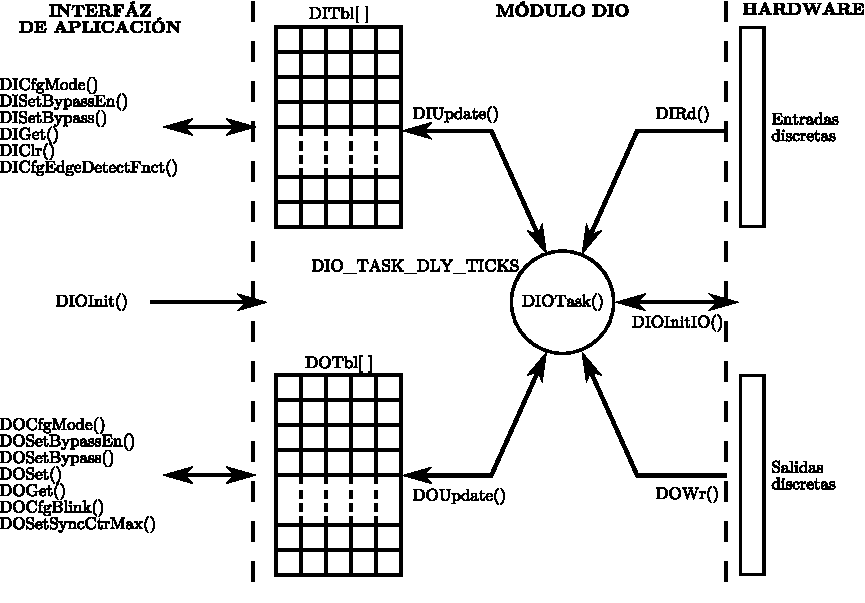
\includegraphics[width=0.8\textwidth]{images/dio_modulo_func}
  \caption{Diagrama de flujo del Módulo DIO.}
  \label{fig:dio-diagrama}
\end{figure}

%\newpage{}
El diagrama en bloque de la Figura \ref{fig:dio-input} muestra el funcionamiento del módulo DIO para el tratado de las señales de entrada. \emph{.DIIn}, \emph{.DIModeSel}, \emph{.DIBypassEn} y \emph{.DIVal} son miembros de la estructura de datos \emph{DIO\_DI} que se encuentra definida en el código fuente del módulo dio (archivo \texttt{DIO.H}). \emph{DIUpdate()} es el responsable de actualizar todas los canales de entradas discretas del módulo.

\begin{figure}[h]
  \centering
  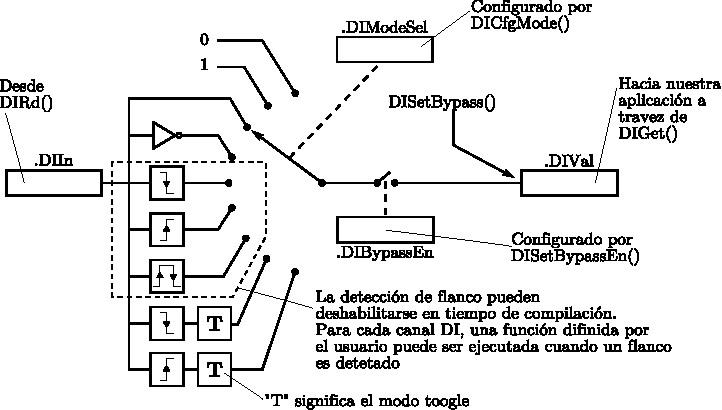
\includegraphics[width=0.8\textwidth]{images/dio_input}
  \caption{Canales de entradas discretas del Módulo DIO.}
  \label{fig:dio-input}
\end{figure}

Al igual que los canales de entrada, Figura \ref{fig:dio-diagrama}, \emph{DOTbl[ ]} es una tabla que contiene configuración e información en tiempo real por cada canal de salidas. Las salidas discretas son mapeadas desde \emph{DOTbl[i].DOOut} al puerto físico a través de la función \emph{DOWr()}. La función \emph{DOWr()} es el controlador o \textsl{driver} que interacciona con la capa física de nuestro sistema (al igual que \emph{DIRr()}). En la Figura \ref{fig:dio-output} se muestra un diagrama de como funciona el módulo DIO para las señales de salida de nuestro bloque. \emph{.DOCtrl}, \emph{.DOBypassEn}, \emph{.DOBypass}, \emph{.DOBlinkEnSel}, \emph{.DOModeSel}, \emph{.DOInv} y \emph{.DOOut} son miembros de la estructura de datos \emph{DIO\_DO} definido en el archivo \texttt{DIO.H}. \emph{DOUpdate()} es el responsable de actualizar todos los canales de salidas discretas.

\begin{figure}[h]
  \centering
  \includegraphics[width=0.85\textwidth]{images/dio_output}
  \caption{Canales de salidas discretas del Módulo DIO.}
  \label{fig:dio-output}
\end{figure}

Como toda tarea que debe atender el RTOS, se debe asignar una prioridad y una latencia en ejecución. Se asigna una de las más altas prioridades al módulo pues será quién controle el sensor. Las además tareas planteadas en la Sección \ref{sec:tareas-rtos} no son tan demandantes. En el caso de especificar a que frecuencia debe ejecutarse el módulo DIO, se considera el valor más alto, lo que implica que se refrescará las Entradas/Salidas lo más rápido posible. El archivo \texttt{DIO.H} contiene varios \#define que parametrizan el comportamiento del módulo.

\begin{lstlisting}[caption={Definiciones de parámetros de prioridad y latencia del Módulo DIO.}]
#define  DIO_TASK_PRIO              1
#define  DIO_TASK_DLY_TICKS         1
\end{lstlisting}

Como se dijo anteriormente, las funciones \emph{DOWr()} y \emph{DIRd()} serán quienes interactúen con el \textsl{hardware}. Originalmente el código del módulo DIO estaba escrito para acceder al puerto paralelo de una computadora de escritorio. La configuración de los puertos del microcontrolador se realiza en la función \emph{DIOInitIO()}, 
\begin{lstlisting}[caption={Función \emph{DIOInitIO()}},label=code:func-dioinitio]
  void  DIOInitIO (void)
  {
    /* Configuración de los puertos I/O */
    /* SALIDAS */
    TRISBbits.TRISB9 = 0;
    TRISBbits.TRISB8 = 0;
    TRISBbits.TRISB7 = 0;
    TRISBbits.TRISB6 = 0;

    /* ENTRADAS */
    TRISCbits.TRISC0 = 1;
    TRISCbits.TRISC1 = 1;
    TRISCbits.TRISC2 = 1;
    TRISCbits.TRISC3 = 1;

    AD1PCFGLbits.PCFG6 = 1;	//RC0
    AD1PCFGLbits.PCFG7 = 1;	//RC1
    AD1PCFGLbits.PCFG8 = 1;	//RC2
  }
\end{lstlisting}

Una vez configurados los puertos, la función \emph{DIOInitIO()} es llamada desde la función principal. La función \emph{DIRd()} es modificada para asignar los puertos que serán leídos y cargados en la tabla \emph{DITbl[ ]}.

\begin{lstlisting}[caption={Función \emph{DIRd()}},label=code:func-dird]
  void  DIRd (void)
  {
    DIO_DI  *pdi;
    INT8U    i;
    INT8U    in;
    INT8U    msk;
    
    pdi = &DITbl[0]; /* Point at beginning of discrete inputs */
    msk = 0x01; /* Set mask to extract bit 0 */
    in = 0;
    in  |= PORTCbits.RC0; /* Read the physical port (8 bits) */
    in  |= (PORTCbits.RC1<<1);           
    in  |= (PORTCbits.RC2<<2);
    in  |= (PORTCbits.RC3<<3);
    for (i = 0; i < 8; i++) /* Map all 8 bits to first 8 DI channels */
    {     
      pdi->DIIn   = (BOOLEAN)(in & msk) ? 1 : 0;
      msk       <<= 1;
      pdi++;
    }
  }
\end{lstlisting}

Recordemos que el módulo DIO puede controlar hasta 256 canales de entradas y salidas. En nuestro caso no se requería de más de dos canales, uno de entrada y otro de salida. De todas formas se configuran cuatro canales I/O. Para la función que escribe el puerto de salida del microcontrolador, \emph{DOWr()}, se debe asignar que puertos físicos tomarán los valores de la tabla \emph{DOTbl[ ]}. Al igual que en el caso de la lectura, aquí se utilizaron solo cuatro canales de los que dispone el módulo DIO.

\begin{lstlisting}[caption={Función \emph{DIWr()}},,label=code:func-dowr]
  void  DOWr (void)
  {
    DIO_DO  *pdo;
    INT8U    i;
    INT8U    out;
    INT8U    msk;
    
    
    pdo = &DOTbl[0]; /* Point at first discrete output channel */
    msk = 0x01; /* First DO will be mapped to bit 0 */
    out = 0x00; /* Local 8 bit port image */
    for (i = 0; i < 8; i++) /* Map first 8 DO to 8 bit port image */
    {
      if (pdo->DOOut == TRUE) {
        out |= msk;
      }
      msk <<= 1;
      pdo++;
    }
    PORTBbits.RB9 = out & 0x01;
    PORTBbits.RB8 = (out>>1) & 0x01;
    PORTBbits.RB7 = (out>>2) & 0x01;
    PORTBbits.RB6 = (out>>3) & 0x01;
  }
\end{lstlisting}

\section{Tarea para el control del sensor}
\label{sec:tarea-sensor}

En la Sección \ref{sec:funcionamiento} se describe el funcionamiento del sistema de censado que se implementa en el correspondiente trabajo. Las señales que controlan el proceso de adquisición de datos a través de la línea de comunicación son generados por una tarea del \uCOS. La tarea \emph{TareaControlSensor()}  utiliza el módulo DIO para generar la señal de \emph{control}, véase el circuito de la Figura \ref{fig:hw-placa-sensor}. El tiempo de \emph{adquisición} y el tiempo de \emph{espera} es controlado por las funciones de tiempo del RTOS, \emph{}

\begin{lstlisting}[caption={Función de la tarea \emph{TareaControlSensor()}},label=code:func-tareacontrol]
  static  void  TareaControlSensor (void)
  {
    
    // Configuración de canales del módulo DIO
    
    DOCfgMode(0,DO_MODE_DIRECT,0);
    DICfgMode(0,DI_MODE_EDGE_HIGH_GOING);
    ValChZero = 0;
    CntData = 0;
    DIClr(0);
    
    while(1)
    {
      
      DOSet(0,TRUE);
      OSTimeDlyHMSM(0,0,0,100);
      DOSet(0,FALSE);
      OSTimeDlyHMSM(0,0,1,0);
      
      ValChZero += DIGet(0);
      CntData++;
      DIClr(0);
      
    }
}
\end{lstlisting}

La salida del microcontrolador que maneja la señal de control del sensor será el primer canal del módulo DIO (canal 0). En esta función se puede apreciar que el tiempo de \emph{adquisición} es 100 microsegundos y el tiempo de \emph{espera} es de 1 segundo, relación especificada en la Sección \ref{sec:funcionamiento}. 

La entrada será el canal 0 y es conectada a la señal de salida del sensor (colector del transistor $Q2$, Fig. \ref{fig:hw-placa-sensor}). Este canal se configura en el modo de detección de flanco ascendente, \emph{DICfgMode(0,DI\_MODE\_EDGE\_HIGH\_GOING)}. Se acumula en la variable \emph{ValChZero} la cantidad de flancos recibidos desde la línea de comunicación y a la vez se acumula el número de muestras recibidas, pues se enviará un promedio del periodo calculado.  Se aclara que la mayoría de las variables que se utilizan en este proyecto son variables globales. La declaración de estas variables se pueden ver al final del documento donde se proporciona todo el código fuente del proyecto.

\section{Tarea procesamiento de datos del sensor}
\label{sec:tarea-proces-datos}

La tarea \emph{TareaPromDatos()} realiza un promedio de la cantidad de pulsos recibidos. La tarea procesa la cantidad de flancos recibidos, que son acumulados en la variable \emph{ValChZero}, y los promedia con la cantidad de veces que se realiza la captura, \emph{CntData}. Este proceso se realiza a una frecuencia menor que la tarea \emph{TareaControlSensor()}, cada 4 segundos. 

En esta función se implementan los \emph{MailBoxes} para comunicarse con la tarea que envíe los datos por el puerto serie. Los \emph{MailBoxes} son recursos que ofrece el \uCOS para intercambiar mensajes entre tareas a través del \textsl{kernel}. Una tarea que desee un mensaje desde un \emph{MailBox} vacío es suspendida y puesta en una lista de espera hasta que el mensaje sea recibido. El \textsl{kernel} permite que la tarea espere por el mensaje hasta que haya transcurrido un tiempo determinado (\textsl{timeout}). Si el mensaje no es recibido, transcurrido el tiempo de espera, la tarea que requiere del mensaje  pasará del estado \emph{Ready} a \emph{Run} retornará un código de error en el retorno del pedido. El mecanismo con el que funciona este servicio de mensajería del sistema operativo se puede ver en al Figura \ref{fig:mailbox}. La función \emph{OSMboxPost()} realiza la acción de \textbf{poner} el mensaje que en este caso es el valor promedio de los datos adquiridos. El primer argumento de la función \emph{OSMboxPost()}, \emph{mBoxPromData}, es una variable del tipo \emph{OS\_EVENT} que es una estructura de datos definida por el \uCOS para el manejo de información interna del sistema operativo. 

\begin{lstlisting}[caption={Función de la tarea \emph{TareaPromDatos()}},label=code:func-tareaprom]
  static  void  TareaPromDatos (void)
  {
    TRISBbits.TRISB5 = 0;
    
    while(1)
    {
      if(CntData!=0)
      {
        Prom = (float) ValChZero / (float) CntData;
        ValChZero = 0;
        CntData = 0;
      }
      else
      {
        Prom = 0;
      }
      
      OSMboxPost(mBoxPromData, &Prom); /* Envío msj. a tarea que transmite los datos (promedio de los pulsos recibidos) */

      OSTimeDlyHMSM(0,0,4,0);
    }
  }
\end{lstlisting}

\begin{figure}[h]
  \centering
  \includegraphics[width=0.5\textwidth]{images/mailbox}
  \caption{Funcionamiento de los \emph{MailBoxes}.}
  \label{fig:mailbox}
\end{figure}

\section{Tarea de comunicación serial}
\label{sec:tarea-com-serial}

La últimas de las tareas implementadas en el microcontrolador es la comunicación serial a través de la UART del dsPIC\textsuperscript{\textregistered}. La configuración de la UART se realiza en la función \emph{InitUART()}. La tarea \emph{TareaComSerial()} se encuentra condicionada a la recepción del mensaje desde la tarea \emph{TareaPromDatos()} a través del \emph{MailBox mBoxPromData}. El tiempo de espera por el mensaje se define en \emph{TIMEOUT\_PEND\_MBOX} y se encuentra en unidades ticks. Una vez que se reciba el mensaje, \emph{OSMboxPend()} proporciona un puntero a la posición de memoria donde se encuentra el mensaje. Y sobre esta información se procesa el dato a ser enviado por el canal serial. La frecuencia con que trabaja esta tarea es de un segundo, pero como se dijo al comienzo, se encuentra condicionada por la espera del \emph{MailBox}.

\begin{lstlisting}[caption={Función de la tarea \emph{TareaComSerial()}},label=code:func-tareacom]
  static  void  TareaComSerial (void)
  {
    uint8_t errorMboxPend;
    
    asm volatile (``mov #OSCCONL, w1  \n''
    ``mov #0x46, w2     \n''
    ``mov #0x57, w3     \n''
    ``mov.b w2, [w1]    \n''
    ``mov.b w3, [w1]    \n''
    ``bclr OSCCON, #6'');
    
    RPINR18bits.U1RXR = 22;
    RPOR11bits.RP23R = 0b00011;
    
    asm volatile (``mov #OSCCONL, w1  \n''
    ``mov #0x46, w2     \n''
    ``mov #0x57, w3     \n''
    ``mov.b w2, [w1]    \n''
    ``mov.b w3, [w1]    \n''
    ``bset OSCCON, #6'');
    
    InitUART1();
    
    while(1)
    {
      PtrPromFromMBox = OSMboxPend(mBoxPromData, TIMEOUT_PEND_MBOX, &errorMboxPend); /* Esperamos a que llegue un nuevo promedio */
      PromFromMbox = *PtrPromFromMBox;
      whole=(int) PromFromMbox ; /* obtains whole part */
      decimal=(int) ((PromFromMbox - (float) whole)*100.0); /* obtains decimal part (1 digit) */
      sprintf(array,":%04d.%02d\n",whole,decimal); /* converts to string */
      for(iiTaskUart = 0; iiTaskUart<9 ; iiTaskUart++)
      {
        while(U1STAbits.UTXBF != 0);
        U1TXREG = array[iiTaskUart];
      }
      
      OSTimeDlyHMSM(0,0,1,0);
      
    }
  }
\end{lstlisting}

\chapter{\uCOS en la PC}
\label{sec:ucos-pc}

Siguiendo la línea del uso de los sistemas operativos en tiempo real, se implementa el sistema \uCOS en una arquitectura de PC estándar. Se utilizará un proyecto base publicado por Micri$\mu$m Inc., creador del \uCOS, compilado con el \textsl{software} \emph{TurboC}. Las características del proyecto serán,

\begin{itemize}
\item Procesar los datos recibidos a través de una comunicación serial con el RTOS que corre en el dsPIC\textsuperscript{\textregistered}. 
\item Manejo de funciones gráficas para la presentación de los datos en la pantalla de la PC.
\end{itemize}

\begin{figure}[h]
  \centering
  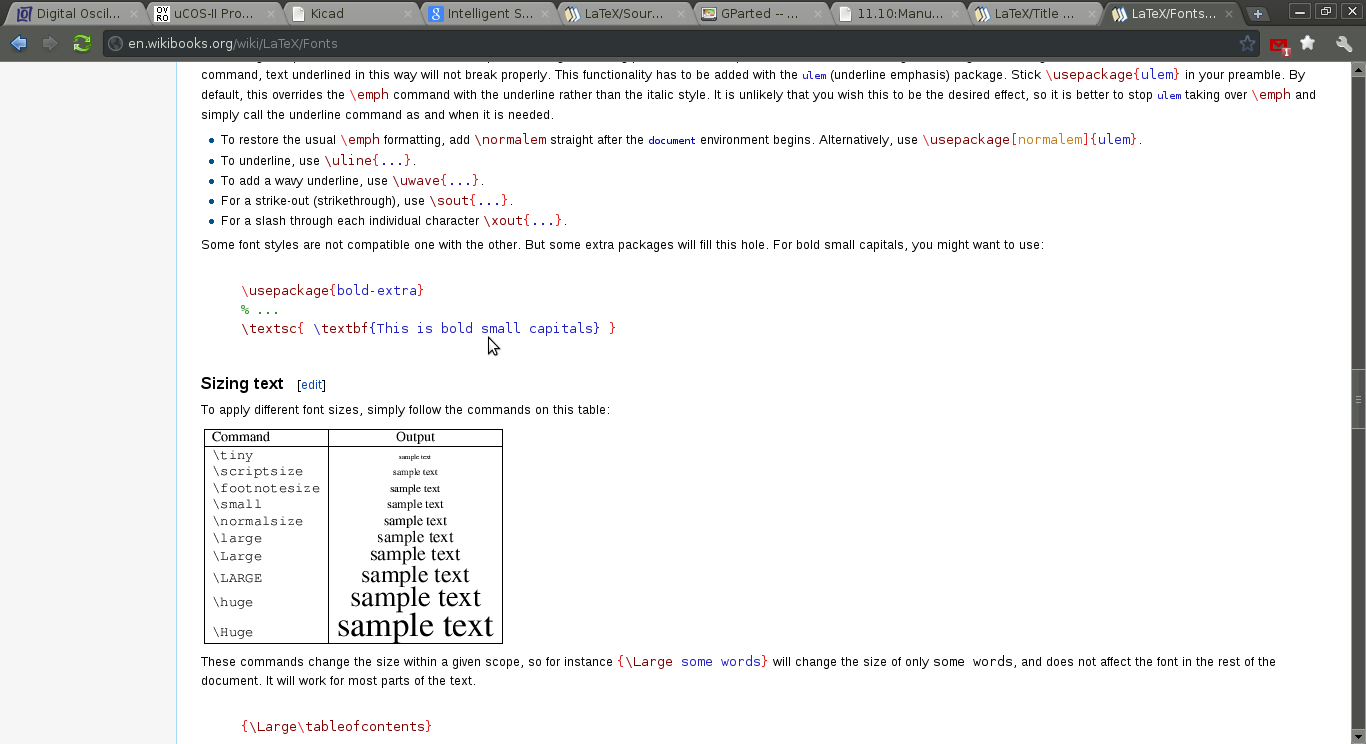
\includegraphics[width=\textwidth]{images/ide-turboc}
  \caption{Entorno gráfico del \textsl{software} TurboC.}
  \label{fig:turboc}
\end{figure}

La función principal \emph{main()} se puede ver en el Código \ref{code:main-pc}. Como en el caso del \uCOS en el dsPIC\textsuperscript{\textregistered}, se debe realiza la configuración y la creación de las tareas luego del llamado a la función \emph{OSInit()} y antes de que el RTOS comience a correr \emph{OSStart()}.

\begin{lstlisting}[caption={Función principal del \uCOS sobre la PC (\emph{main()})},label=code:main-pc]
  void main (void)
  {
    PC_DispClrScr(DISP_FGND_WHITE); /* Clear the screen */

    OSInit(); /* Initialize uC/OS-II */

    PC_DOSSaveReturn(); /* Save environment to return to DOS */
    PC_VectSet(uCOS, OSCtxSw); /* Install uC/OS-II's context switch vector */
    PC_ElapsedInit(); /* Initialized elapsed time measurement  */
    
    CommInit();

    /* Crear los Semaphores (Buzones) */
    TransmisionesListasSem = OSSemCreate(0);
    
    /*Crear los MailBox (Buzones) */
    DatoRecibidoMbox=OSMboxCreate((void *)0);
    
    OSTaskCreate(TaskStart, (void *)0, &TaskStartStk[TASK_STK_SIZE-1], 0);
    
    OSStart(); /* Start multitasking   */
  }
\end{lstlisting}

Junto a los archivos del \uCOS se dispone de varios códigos fuentes para hacer uso de varios periféricos. Estos se encuentran en el directorio \emph{BLOCKS}. Se puede  listar estos archivos como,

\dirtree{%
.1 SOFTWARE.
.2 BLOCKS.
.3 AIO.   
.3 CLK.   
.3 \textbf{COMM}. .4 SOURCE. .5 COMMRTOS.H. .5 COMMRTOS.C. .5 COMM\_PC.H. .5 COMM\_PC.C. .5 COMM\_PCA.ASM. .5 COMMBGND.H. .5 COMMBGND.C.  
.3 DIO.   
.3 KEY\_MN.
.3 LCD.   
.3 LED.   
.3 \textbf{PC}. .4 SOURCE. .5 PC.C. .5 PC.H.
.3 SIMPLE.
.3 TMR.    
.2 HPLISTC.
.2 UCOS-II.
.2 doc.
}

Los bloques que se utilizarán se encuentran resaltados en texto negrita. Pero también se puede ver el módulo DIO utilizado en el dsPIC\textsuperscript{\textregistered} también está listado en este directorio. 

Para el manejo de la pantalla se utilizan funciones del módulo \emph{PC}. Este módulo provee servicios para mostrar caracteres ASCII en una pantalla VGA básica de una computadora. En el modo normal, la pantalla de una PC puede manejar hasta 2000 caracteres organizados en un arreglo de 25 filas por 80 columnas. La memoria de vídeo en la PC y comienza en una dirección absoluta de memoria 0x000B8000 (o usando notación segmentada, B800:0000). Cada caracter  a mostrar requiere dos \textsl{bytes} para ser visualizado en la pantalla. El primer \textsl{byte} (menor posición en memoria) es el caracter que se quiere mostrar, mientras que el segundo \textsl{byte} es un atributo que determina la combinación de color \textsl{foreground}/\textsl{background} del caracter. El color \textsl{foreground} es especificado en los menores 4 \textsl{bits} del atributo, mientras que el color \textsl{background} en los superiores, del \textsl{bits} 4 al 6. Finalmente el más significativo \textsl{bit} determina si el caracter titilará (con 1)  o no (con 0).

El el Código \ref{code:pc-taskstart} muestra la primer tarea donde se configura y ejecuta varias llamadas a las funciones de pantalla para nuestro proyecto. 

\begin{lstlisting}[caption={Primera tarea del \uCOS sobre la PC (\emph{TaskStart()})},label=code:pc-taskstart]
  void  TaskStart (void *data)
  {
    char   s[80];
    WORD key;
    
    data = data; /* Prevent compiler warning */
    
    OS_ENTER_CRITICAL(); /* Install uC/OS-II's clock tick ISR */
    PC_VectSet(0x08, OSTickISR);
    PC_SetTickRate(OS_TICKS_PER_SEC); /* Reprogram tick rate  */
    OS_EXIT_CRITICAL();
    OSStatInit();
    
    OSTaskCreate(Task_Times, (void *)0, &TaskTimesStk[TASK_STK_SIZE-1], 7);
    OSTaskCreate(Task_Rx, (void *)0, &TaskRxStk[TASK_STK_SIZE-1], 8);
    
    
    for (;;)
    {
      PC_DispStr(16,  1, "Trabajo Final - uC/OS-II, The Real-Time Kernel", DISP_FGND_WHITE + DISP_BGND_RED + DISP_BLINK);
      PC_DispStr(25, 27, "<-PRESS 'ESC' TO QUIT->", DISP_FGND_WHITE + DISP_BLINK);
      if (PC_GetKey(&key)== TRUE)	/* See if key has been pressed */
      {
        if (key == 0x1B) /* Yes, see if it's the ESCAPE key */
        {
          PC_DOSReturn(); /* Yes, return to DOS */
        }
      }
      OSTimeDlyHMSM(0, 0, 0, 200);
    }
  }  
\end{lstlisting}

En la primera tarea se crean las demás tareas del \uCOS. En este caso son, la tarea que realiza la recepción de datos a través del puerto serie y última es una tarea que realiza la limpieza de la pantalla. Una captura de la pantalla se observa en la Figura \ref{fig:captura-pantalla-ucos}. 


\begin{figure}[h]
  \centering
  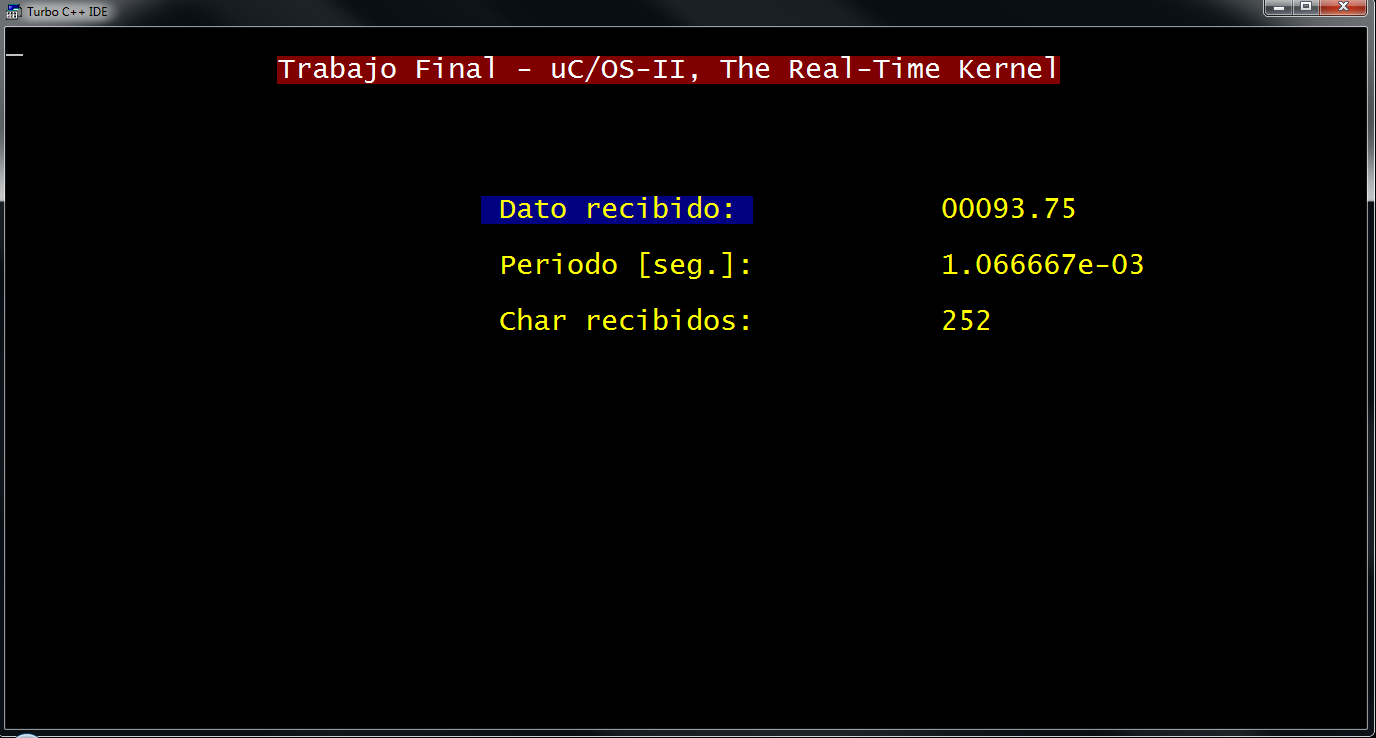
\includegraphics[width=\textwidth]{images/captura-pantalla-ucos}
  \caption{Captura de la pantalla del proyecto en funcionamiento.}
  \label{fig:captura-pantalla-ucos}
\end{figure}

\section{Tarea de comunicación serial}
\label{sec:mod-com}

Para manejar el interfaz serial de la PC se hace uso de un módulo proporcionado por el autor del \uCOS, el \emph{COMM\_PC}. Este módulo hace mucho más fácil de usar el puerto serie. El código y sus funcionalidades del \textsl{driver} son fácilmente portable a diferentes arquitecturas y entornos de desarrollo. La estructura del módulo cuenta con dos bloques como se muestra en la Figura \ref{fig:comm-pc}. El bloque \textsl{Low Level PC Driver} es responsable de interactuar con el \textsl{hardware}, es decir, la UART de la PC. Se provee de funciones a nuestras aplicaciones que nos permitan configurar los dos puertos (\emph{COM1} ó \emph{COM2}), habilitar/deshabilitar interrupciones de comunicación, y adquirir/cargar el vector de interrupción del puerto \emph{COM}.
Nuestras aplicaciones también interaccionan a dos posibles tipos de \textsl{buffers} seriales, los módulos de I/O: \emph{COMMBGND} ó \emph{COMMRTOS}. Se puede usar el código del \emph{COMMBGND} en aplicaciones \textsl{foreground}/\textsl{background} y el \emph{COMMRTOS} si se está utilizando un \textsl{kernel}en tiempo real como el \uCOS.

\begin{figure}[h]
  \centering
  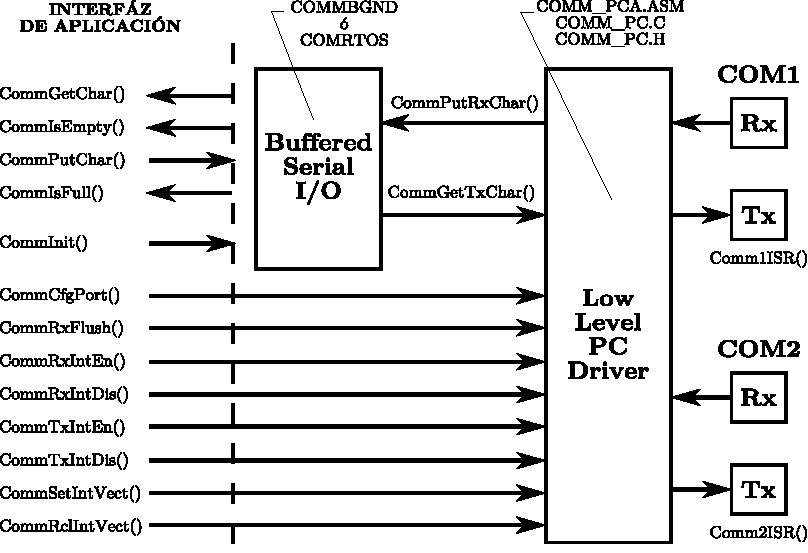
\includegraphics[width=0.6\textwidth]{images/modulo_comm_pc}
  \caption{Diagrama en bloque del Módulo \emph{COMM\_PC}.}
  \label{fig:comm-pc}
\end{figure}

Se podría describir en detalle el funcionamiento del módulo \emph{COMM\_PC} pero no es la finalidad del presente informe. La documentación completa sobre este módulo se encuentra descrito en detalle en el libro \emph{Embedded Systems Building Blocks, Second Edition} escrito por el \emph{Jean  J. Labrosse}.

La comunicación es unidireccional, por las especificaciones del proyecto, pero para realizar una comunicación bidireccional no ha de ser inconveniente. En el Código \ref{code:pc-task-rx} antes de lanzar el bucle infinito de la tarea, se configura el puerto serie de la PC, \emph{CommCfgPort(COMM2,9600,8,COMM\_PARITY\_NONE,1)}. Y se lanza las interrupciones del puerto COMM2. Ya en tiempo de ejecución, se espera a que el \textsl{buffer} del puerto serie se encuentre con datos a ser procesados y son almacenados temporalmente para ser visualizados con los servicios de pantalla de la función \emph{PC\_DispStr()}. Además en esta tarea se utiliza \emph{MailBox}, recursos de comunicación interna entre tareas que ofrece el \uCOS. Aquí el \emph{MailBox} \emph{DatoRecibidoMbox} envía la trama recibida a la tarea de visualización. Esta trama de datos está identificada  por un caracter de comienzo ``:'' (en decimal 58), y uno de final de trama ``\\n'' (en decimal 10).

\begin{lstlisting}[caption={Tarea de la recepción de datos en la PC (\emph{Task\_Rx()})},label=code:pc-task-rx]
void Task_Rx (void *data)
{
  INT8U	error, errSem,errMbox;
  INT8U	i, c;
  INT8U	periodo[7],s[8];
  int k=0,kk=0 ,kdata = 0;
  char sdata[] = "0000.00";
  INT8U	FlagInicio = 0;
  
  data = data;
  
  CommCfgPort(COMM2,9600,8,COMM_PARITY_NONE,1);
  CommSetIntVect(COMM2);
  CommRxIntEn(COMM2);
  
  for(;;)
  {
    PC_DispStr(28, 6, " Dato recibido: ", DISP_FGND_YELLOW + DISP_BGND_BLUE);
    PC_DispStr(28, 8, " Periodo [seg.]: ", DISP_FGND_YELLOW);
    PC_DispStr(28, 10, " Char recibidos: ", DISP_FGND_YELLOW);
    
    if(!CommIsEmpty(COMM2))
    {
      c = CommGetChar(COMM2,&error);
      if(error==COMM_NO_ERR)
      {
        switch(c)
        {
          case 58:
          FlagInicio = 1;
          break;
          case 10:
          kdata = 0;
          FlagInicio = 0;
          errMbox = OSMboxPost(DatoRecibidoMbox, (void *)&sdata[0]);
          break;
          default:
          if(FlagInicio == 1)
          {
            k++;
            kdata++;
            sprintf(s, "%d", k);
            PC_DispStr(55, 10, s, DISP_FGND_YELLOW);
            sdata[kdata] = c;
          }
        }
      }
    }
    
    OSTimeDlyHMSM(0, 0, 0, 100);
  }
}

\end{lstlisting}


\section{Tarea visualización de datos}
\label{sec:limpieza-pantalla}

Esta tarea es muy sencilla de interpretar. Aquí se espera a que se haya recibido una trama completa en la tarea \emph{Task\_Rx}, pues se espera por el \emph{MailBox}. A la vez que se escriben los datos en la pantalla, se calcula el periodo en unidades de segundos y también es visualizada. .

\begin{lstlisting}[caption={Tarea de limpieza de pantalla (\emph{Task\_DispData()})},label=code:pc-task-clrdisp]
  void  Task_DispData(void *data)
  {
	INT8U	err;
	INT8U 	errSem,errMbox;
	char 	s[40];
	char *PtrSData;
	float  Fdata,periodo;
	data = data;

	for (;;)
	{

		PtrSData = OSMboxPend(DatoRecibidoMbox,0,&errMbox);

		PC_DispStr(55, 6, PtrSData, DISP_FGND_YELLOW);

		Fdata = atof(PtrSData);

		if(Fdata == 0.0)
			periodo = 0.0;
		else
			periodo = 0.1 / Fdata;

		sprintf(s, "%e", periodo);
		PC_DispStr(55, 8, s, DISP_FGND_YELLOW);

		//PC_DispClrScr(DISP_FGND_WHITE);
		//clrscr();

		OSTimeDlyHMSM(0, 0, 0, 100);      /* Espera 1 Segundo   */
	}
  }
\end{lstlisting}

\chapter{Ensayos}
\label{sec:ensayos}

Los ensayos realizados sobre todo el sistema funcionando son principalmente sobre el sistema de comunicación entre el \emph{Sensor} y el bloque de \emph{Control}. La forma de las señales sobre el canal serial en el caso ideal se observan en la Figura \ref{fig:ciclo-tiempo}. Para realizar el testeo del sistema se ha utilizado un \textsl{Dimmer} que nos permitirá modificar la intensidad de luz que incide sobre el sensor fotoeléctrico. La Tabla \ref{tab:ensayo-muestras} presenta varias mediciones realizadas a diferentes niveles de atenuación del \textsl{Dimmer}. Se contrasta el periodo adquirido por el dsPIC\textsuperscript{\textregistered} (segunda columna) y la medición del mismo con un osciloscopio. (tercera columna).

\begin{table}[H]
   \centering
   \begin{tabular}[h]{|c|r|r|}
     \hline
     \multirow{2}{*}{\textbf{Muestra}}  & \multicolumn{2}{|c|}{\textbf{Periodo}} \\
     \cline{2-3}
     & \textbf{dsPIC\textsuperscript{\textregistered}} & \textbf{Medido} \\
     \hline
     Muestra 1 & 3.5  & 368 $\mu$seg. \\
     \hline
     Muestra 2 & 29.5 & 2873 $\mu$seg. \\
     \hline
     Muestra 3 & 85   & 8622 $\mu$seg. \\
     \hline
     Muestra 4 & 120  & 12.1 $\mu$seg. \\
     \hline
%     última muestra & OSC\\
   \end{tabular}
   \caption{Captura de datos del sistema de sensor a diferentes niveles de intensidad de luz.}
   \label{tab:ensayo-muestras}
\end{table}

Por último se muestran las capturas desde el osciloscopio para las diferentes muestras presentadas en la Tabla \ref{tab:ensayo-muestras}.

\begin{figure}[H]
  \begin{subfigure}[b]{\textwidth}
    \centering
    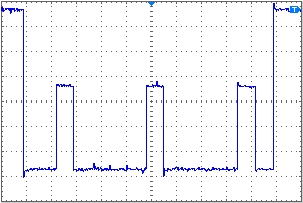
\includegraphics[width=0.45\textwidth]{images/line_periodo_1}
    \subcaption{Señales tomadas sobre la línea de comunicación del sensor/control.}\label{fig:line-per-1}
  \end{subfigure}
%  \hfill
  \begin{subfigure}[b]{\textwidth}
    \centering
    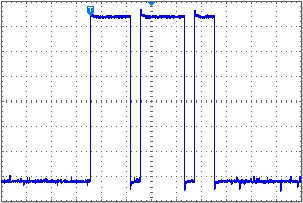
\includegraphics[width=0.45\textwidth]{images/out_periodo_1}
    \subcaption{Señales tomadas en la salida del sistema de control (colector $Q2$).}\label{fig:out-per-1}
  \end{subfigure}
  \caption{Muestra 1.}
  \label{fig:muestra1}
\end{figure}

\begin{figure}[H]
  \begin{subfigure}[b]{\textwidth}
    \centering
    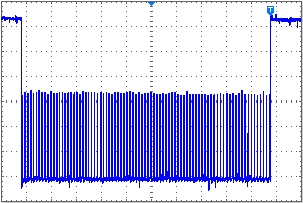
\includegraphics[width=0.45\textwidth]{images/line_periodo_2}
    \subcaption{Señales tomadas sobre la línea de comunicación del sensor/control.}\label{fig:line-per-2}
  \end{subfigure}
%  \hfill
  \begin{subfigure}[b]{\textwidth}
    \centering
    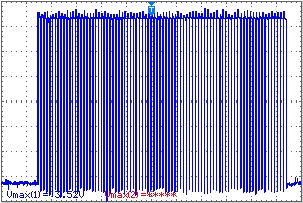
\includegraphics[width=0.45\textwidth]{images/out_periodo_2}
    \subcaption{Señales tomadas en la salida del sistema de control (colector $Q2$).}\label{fig:out-per-2}
  \end{subfigure}
  \caption{Muestra 2.}
  \label{fig:muestra1}
\end{figure}

\begin{figure}[H]
  \begin{subfigure}[b]{\textwidth}
    \centering
    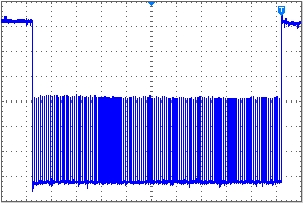
\includegraphics[width=0.45\textwidth]{images/line_periodo_3}
    \subcaption{Señales tomadas sobre la línea de comunicación del sensor/control.}\label{fig:line-per-3}
  \end{subfigure}
%  \hfill
  \begin{subfigure}[b]{\textwidth}
    \centering
    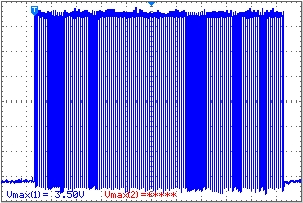
\includegraphics[width=0.45\textwidth]{images/out_periodo_3}
    \subcaption{Señales tomadas en la salida del sistema de control (colector $Q2$).}\label{fig:out-per-3}
  \end{subfigure}
  \caption{Muestra 3.}
  \label{fig:muestra1}
\end{figure}

\appendix{}

\chapter{Repositorio del proyecto}
\label{sec:rep-proy}

El proyecto se encuentra bajo en control de versiones proporcionado por el \textsl{software} \emph{Subversion}, conocido también con las siglas \emph{SVN}. Este proyecto como su código fuente y documentación se encuentra publicado bajo \emph{Licencias Libre} para su uso y modificación. Para acceder al proyecto, bajo sistemas operativos GNU/Linux \& Unix, simplemente se corre el comando,

\begin{lstlisting}[language=bash]
svn checkout http://proyecto5r1.googlecode.com/svn/branches/ProyectoSensorConUCOSII/firmware proyectosensorconucosii-read-only
\end{lstlisting}

El proyecto es una ramificación de un proyecto ya ralizado por los estudiantes \emph{Andrés Hoc} y \emph{Gonzalo Vassia} quienes han decidido publicar su proyecto también en forma libre. Para conocer más sobre el manejo de repositorios \emph{SVN} y como se realizan proyectos a partir de una raiz (\emph{trunk}) acceda a la documentación de la siguiente página web: \texttt{http://svnbook.red-bean.com/en/1.6/svn.intro.whatis.html}.

\chapter{Códigos del proyecto}
\label{sec:cod-proyectos}

Se adjuntan los códigos fuentes de los archivos más importantes del proyecto. De todas formas este puede ser accedido desde el repositorio. 

\lstinputlisting[language=C,basicstyle=\ttfamily\tiny,breaklines=true, title=\lstname]{../../v0.1/app.c}

\lstinputlisting[language=C,basicstyle=\ttfamily\tiny,breaklines=true, title=\lstname]{../../v0.1/app_cfg.h}

\lstinputlisting[language=C,basicstyle=\ttfamily\tiny,breaklines=true, title=\lstname]{../../v0.1/dsPIC_a.s}

\lstinputlisting[language=C,basicstyle=\ttfamily\tiny,breaklines=true, title=\lstname]{../../v0.1/dsPIC_cfg.c}

\lstinputlisting[language=C,basicstyle=\ttfamily\tiny,breaklines=true, title=\lstname]{../../v0.1/dsPIC_cfg.h}

\lstinputlisting[language=C,basicstyle=\ttfamily\tiny,breaklines=true, title=\lstname]{../../v0.1/dsPIC_delay.c}

\lstinputlisting[language=C,basicstyle=\ttfamily\tiny,breaklines=true, title=\lstname]{../../v0.1/dsPIC_delay.h}

\lstinputlisting[language=C,basicstyle=\ttfamily\tiny,breaklines=true, title=\lstname]{../../v0.1/globals.c}

\lstinputlisting[language=C,basicstyle=\ttfamily\tiny,breaklines=true, title=\lstname]{../../v0.1/globals.h}

\lstinputlisting[language=C,basicstyle=\ttfamily\tiny,breaklines=true, title=\lstname]{../../v0.1/includes.h}

\lstinputlisting[language=C,basicstyle=\ttfamily\tiny,breaklines=true, title=\lstname]{../../v0.1/drivers/DIO/SOURCE/DIO.C}

\lstinputlisting[language=C,basicstyle=\ttfamily\tiny,breaklines=true, title=\lstname]{../../v0.1/drivers/DIO/SOURCE/DIO.H}

\lstinputlisting[language=C,basicstyle=\ttfamily\tiny,breaklines=true, title=\lstname]{../../v0.1/drivers/UART.c}

\lstinputlisting[language=C,basicstyle=\ttfamily\tiny,breaklines=true, title=\lstname]{../../v0.1/drivers/UART.h}

\newpage{}

\lstinputlisting[language=C,basicstyle=\ttfamily\tiny,breaklines=true, title=\lstname]{/media/sda2/SOFTWARE/UCOS-II/TFINAL/TFINAL.C}

\lstinputlisting[language=C,basicstyle=\ttfamily\tiny,breaklines=true, title=\lstname]{/media/sda2/SOFTWARE/UCOS-II/TFINAL/INCLUDE.H}

\lstinputlisting[language=C,basicstyle=\ttfamily\tiny,breaklines=true, title=\lstname]{/media/sda2/SOFTWARE/UCOS-II/TFINAL/OS_CFG.H}

\end{document}
